% !TEX program = xelatex
% ============================================================
%  机器学习 · 讲义  第六讲：决策树
%  海军深蓝 · 经典学术版式
%  编译：xelatex 06_decision_tree.tex
%        （无 .aux 时连跑三遍；已有中间文件时两遍即可）
% ============================================================
\documentclass[11pt,a4paper,fontset=windows,zihao=-4]{ctexart}

% ---------- 版面 ----------
\usepackage{geometry}
\geometry{a4paper,left=2.55cm,right=2.55cm,top=2.55cm,bottom=2.45cm,
  headheight=18pt,headsep=0.52cm,footskip=0.95cm,
  marginparsep=0.40cm,marginparwidth=2.10cm}

% ---------- 数学与字体 ----------
\usepackage{amsmath,amssymb,amsthm,mathtools}
\usepackage{newpxtext,newpxmath}
\usepackage{microtype}

% ---------- 颜色 ----------
\usepackage[table]{xcolor}
\definecolor{navy}{HTML}{0B2545}      % 海军深蓝（主色）
\definecolor{navy2}{HTML}{33587A}     % 次级蓝
\definecolor{steel}{HTML}{4A6478}     % 灰蓝
\definecolor{grey}{HTML}{6B7280}      % 中性灰
\definecolor{mist}{HTML}{F4F6F9}      % 极浅蓝灰（底色）
\definecolor{gold}{HTML}{8A6A3B}      % 暗金（仅用于提示）
\definecolor{goldlight}{HTML}{C6A15B} % 亮金（深蓝底上的金线）

% ---------- 表格与列表 ----------
\usepackage{booktabs}
\usepackage{array}
\usepackage{multirow}
\usepackage{enumitem}
\setlist[itemize]{leftmargin=1.6em,topsep=0.45em,itemsep=0.28em,parsep=0pt}
\setlist[enumerate]{leftmargin=2.0em,topsep=0.45em,itemsep=0.28em,parsep=0pt}

% ---------- 图形 ----------
\usepackage{tikz}
\usetikzlibrary{calc,positioning,arrows.meta,decorations.pathreplacing,
  patterns,backgrounds,fit,shapes.geometric}
\usepackage{pgfplots}
\pgfplotsset{compat=1.18}

% ---------- 彩色框 ----------
\usepackage[most]{tcolorbox}

% ---------- 页眉页脚 ----------
\usepackage{fancyhdr}
\usepackage{titlesec}
\usepackage{caption}
\usepackage{marginnote}
\usepackage{tocloft}

% ---------- 超链接 ----------
\usepackage[colorlinks=true,linkcolor=navy,urlcolor=steel,citecolor=navy,
  bookmarksnumbered=true]{hyperref}
\hypersetup{
  pdftitle={机器学习·讲义（第六讲）：决策树},
  pdfauthor={CyArk},
  pdfsubject={递归划分、切分准则与剪枝},
  pdfkeywords={决策树, 基尼, 信息增益, 贪心生长, 代价复杂度剪枝, 稳定性}
}

% ============================================================
%  数学宏
% ============================================================
\newcommand{\R}{\mathbb{R}}
\newcommand{\bx}{\boldsymbol{x}}
\newcommand{\bX}{\mathbf{X}}
\newcommand{\by}{\mathbf{y}}
\newcommand{\bw}{\mathbf{w}}
\newcommand{\ba}{\mathbf{a}}
\newcommand{\bp}{\mathbf{p}}
\newcommand{\bq}{\mathbf{q}}
\newcommand{\bz}{\mathbf{z}}
\newcommand{\btheta}{\boldsymbol{\theta}}
\newcommand{\bphi}{\boldsymbol{\phi}}
\newcommand{\bDelta}{\boldsymbol{\Delta}}
\newcommand{\bSigma}{\boldsymbol{\Sigma}}
\newcommand{\bmu}{\boldsymbol{\mu}}
\newcommand{\bzero}{\mathbf{0}}
\newcommand{\bmone}{\mathbf{1}}
\newcommand{\tp}{^{\top}}
\newcommand{\norm}[1]{\lVert #1\rVert}
\newcommand{\abs}[1]{\lvert #1\rvert}
\DeclareMathOperator*{\argmin}{arg\,min}
\DeclareMathOperator*{\argmax}{arg\,max}
\DeclareMathOperator{\tr}{tr}
\DeclareMathOperator{\Var}{Var}
\DeclareMathOperator{\Bias}{Bias}
\DeclareMathOperator{\SSE}{SSE}
\DeclareMathOperator{\Err}{Err}
\DeclareMathOperator{\SplitInfo}{SplitInfo}
\DeclareMathOperator{\GainRatio}{GainRatio}
\DeclareMathOperator{\MDI}{MDI}
\DeclareMathOperator{\PI}{PI}
\newcommand{\Dcal}{\mathcal{D}}
\newcommand{\Lcal}{\mathcal{L}}
\newcommand{\Rcal}{\mathcal{R}}
\newcommand{\Xcal}{\mathcal{X}}
\newcommand{\Scal}{\mathcal{S}}
\newcommand{\Ucal}{\mathcal{U}}
\newcommand{\Bcal}{\mathcal{B}}
\newcommand{\Ind}{\mathbb{I}}
\newcommand{\dd}{\mathrm{d}}

% ============================================================
%  版式细节
% ============================================================
\linespread{1.30}
\setlength{\parskip}{0.24em}
\setlength{\parindent}{2em}

% 章节样式
\ctexset{
  section/name={},
  section/number=\arabic{section},
}
\titleformat{\section}[block]
  {\normalfont\sffamily\Large\bfseries\color{navy}}
  {\colorbox{navy}{\makebox[1.55em][c]{\color{white}\thesection}}\hspace{0.75em}}{0pt}{}
  [\vspace{0.30em}{\color{navy!30}\titlerule[0.7pt]}]
\titlespacing*{\section}{0pt}{2.4ex plus 1.0ex minus 0.4ex}{1.5ex}

\titleformat{\subsection}[hang]
  {\normalfont\sffamily\large\bfseries\color{navy!88}}
  {\thesubsection}{0.65em}{}
\titlespacing*{\subsection}{0pt}{1.8ex plus 0.6ex}{0.8ex}

\titleformat{\subsubsection}[runin]
  {\normalfont\sffamily\bfseries\color{navy!80}}
  {}{0pt}{}
\titlespacing*{\subsubsection}{0pt}{1.2ex plus 0.4ex}{0.6em}

\titleformat{\paragraph}[runin]
  {\normalfont\sffamily\bfseries\color{navy!88}}
  {}{0pt}{}
\titlespacing*{\paragraph}{0pt}{1.05ex plus 0.35ex}{0.55em}

% 页眉页脚
\pagestyle{fancy}
\fancyhf{}
\renewcommand{\headrulewidth}{0.5pt}
\renewcommand{\headrule}{{\color{navy!40}%
  \hrule height \headrulewidth width \headwidth}}
\fancyhead[L]{\sffamily\footnotesize\color{steel}机器学习\,·\,讲义}
\fancyhead[R]{\sffamily\footnotesize\color{steel}\leftmark}
\fancyfoot[C]{\sffamily\footnotesize\color{navy}\thepage}
\renewcommand{\sectionmark}[1]{\markboth{\thesection\quad #1}{}}
\fancypagestyle{plain}{%
  \fancyhf{}\renewcommand{\headrulewidth}{0pt}%
  \fancyfoot[C]{\sffamily\footnotesize\color{navy}\thepage}}

% 图表标题
\captionsetup{font={small},labelfont={bf,sf,color=navy},labelsep=quad,
  justification=centering,skip=6pt}

% 目录（手工排版标题，避免 \leftmark 捕获颜色命令）
\makeatletter
\renewcommand{\tableofcontents}{%
  \par\begingroup
    \sffamily\Large\bfseries\color{navy}目\quad 录\par
  \endgroup
  \vspace{0.85em}
  \setlength{\parskip}{0pt}%
  \@starttoc{toc}%
}
\makeatother

% 目录条目样式
\renewcommand{\cftsecfont}{\footnotesize\sffamily\bfseries\color{navy}}
\renewcommand{\cftsecpagefont}{\footnotesize\sffamily\bfseries\color{navy}}
\renewcommand{\cftsubsecfont}{\footnotesize\color{navy!85}}
\renewcommand{\cftsubsecpagefont}{\footnotesize\color{navy!85}}
\renewcommand{\cftsubsubsecfont}{\color{steel}}
\renewcommand{\cftsubsubsecpagefont}{\color{steel}}
\renewcommand{\cftsecleader}{\cftdotfill{\cftdotsep}}
\renewcommand{\cftsubsecleader}{\cftdotfill{\cftdotsep}}
\renewcommand{\cftsubsubsecleader}{\cftdotfill{\cftdotsep}}
\setlength{\cftsecnumwidth}{1.9em}
\setlength{\cftsubsecnumwidth}{2.5em}
\setlength{\cftsubsubsecnumwidth}{3.4em}
\setlength{\cftbeforesecskip}{4.0pt}
\setlength{\cftbeforesubsecskip}{0.2pt}
\setlength{\cftbeforesubsubsecskip}{0pt}
\renewcommand{\cftsecaftersnum}{\hspace{0.55em}}
\renewcommand{\cftsubsecaftersnum}{\hspace{0.4em}}
\renewcommand{\cftsubsubsecaftersnum}{\hspace{0.35em}}

% ============================================================
%  提示框样式
% ============================================================
\tcbset{
  basebox/.style={
    enhanced, breakable, sharp corners,
    boxrule=0pt, leftrule=2.2pt, arc=0pt, outer arc=0pt,
    left=0.9em, right=0.9em, top=0.45em, bottom=0.62em,
    before skip=0.85em, after skip=0.85em,
    before upper={\parindent=0pt\parskip=0.35em},
    fonttitle=\sffamily\bfseries\small,
    coltitle=navy, titlerule=0.35pt,
    toptitle=0.32em, bottomtitle=0.5em,
  }
}
\newtcolorbox[auto counter,number within=section]{dfn}[1][]{%
  basebox, colframe=navy, colback=mist, colbacktitle=mist,
  title={定义~\thetcbcounter\quad\textcolor{navy!45}{\textbar}\quad\textcolor{navy}{#1}}}
\newtcolorbox[auto counter,number within=section]{thm}[1][]{%
  basebox, colframe=navy, colback=white, colbacktitle=white,
  title={定理~\thetcbcounter\quad\textcolor{navy!45}{\textbar}\quad\textcolor{navy}{#1}}}
\newtcolorbox[auto counter,number within=section]{prop}[1][]{%
  basebox, colframe=navy2, colback=white, colbacktitle=white,
  title={命题~\thetcbcounter\quad\textcolor{navy!45}{\textbar}\quad\textcolor{navy}{#1}}}
\newtcolorbox[auto counter,number within=section]{exm}[1][]{%
  basebox, colframe=steel, colback=white, colbacktitle=white,
  title={例题~\thetcbcounter\quad\textcolor{steel!45}{\textbar}\quad\textcolor{steel}{#1}}}
\newtcolorbox{add}[1][]{%
  basebox, colframe=steel, colback=mist, colbacktitle=mist,
  title={\textcolor{steel}{补充}\quad\textcolor{steel!45}{\textbar}\quad\textcolor{steel}{#1}}}
\newtcolorbox{warn}[1][]{%
  basebox, colframe=gold, colback=gold!4, colbacktitle=gold!4,
  title={\textcolor{gold}{注意}\quad\textcolor{gold!55}{\textbar}\quad\textcolor{gold}{#1}}}
\newtcolorbox{keybox}[1][]{%
  enhanced, breakable, sharp corners, boxrule=0.55pt,
  colframe=navy!55, colback=navy!3, colbacktitle=navy!3,
  left=0.9em, right=0.9em, top=0.45em, bottom=0.62em,
  before skip=1.0em, after skip=1.0em,
  before upper={\parindent=0pt\parskip=0.35em},
  fonttitle=\sffamily\bfseries\small, coltitle=navy,
  titlerule=0.35pt, toptitle=0.3em, bottomtitle=0.5em,
  title={\textcolor{navy}{#1}}}

% 边注
\renewcommand*{\marginfont}{\footnotesize\color{steel}}
\setlength{\marginparpush}{6pt}

% 常用小工具
\newcommand{\hl}[1]{\textcolor{navy}{\textbf{#1}}}
\newcommand{\tabhead}{\sffamily\bfseries\color{navy}}
\tikzset{
  nd/.style={draw=navy!55,fill=white,sharp corners,inner sep=3pt,
    font=\scriptsize,align=center,line width=0.5pt},
  lf/.style={draw=navy!45,fill=navy!4,sharp corners,inner sep=3pt,
    font=\scriptsize,align=center,line width=0.5pt},
  eg/.style={draw=navy!55,line width=0.55pt},
  cut/.style={draw=navy2,dashed,line width=0.55pt},
  p0/.style={circle,draw=navy,fill=white,inner sep=0pt,minimum size=4.2pt,line width=0.6pt},
  p1/.style={rectangle,fill=navy,draw=navy,inner sep=0pt,minimum size=4.2pt},
  lb/.style={font=\scriptsize,text=steel,inner sep=2pt},
  ax/.style={->,steel!60,line width=0.6pt},
}

\begin{document}

% ============================================================
%  封面 · 目录 · 导读
% ============================================================

\begin{titlepage}
\thispagestyle{empty}
\raggedright
% ---- 顶部深蓝色块 + 金色分隔线 + 树与数轴 ----
\begin{tikzpicture}[remember picture, overlay]
  \fill[navy] (current page.north west) rectangle ([yshift=-12.30cm]current page.north east);
  \fill[goldlight] ([yshift=-12.30cm]current page.north west)
        rectangle ([yshift=-12.37cm]current page.north east);
  % 右侧：例 A 的树与数轴（真实解：3.5 与 6.5 两刀，三片叶）
  \begin{scope}[shift={([xshift=12.30cm,yshift=-10.28cm]current page.north west)}]
    \draw[white,opacity=0.09,line width=0.35pt] (0,0) rectangle (7.02,4.60);
    % 树：节点用圆点，标签置于点下
    \fill[white,opacity=0.92] (3.69,4.30) circle (1.9pt);
    \fill[white,opacity=0.92] (1.53,3.20) circle (1.9pt);
    \fill[white,opacity=0.92] (4.98,3.20) circle (1.9pt);
    \fill[white,opacity=0.92] (3.69,2.15) circle (1.9pt);
    \fill[white,opacity=0.92] (5.86,2.15) circle (1.9pt);
    \node[font=\tiny,text=white,opacity=0.88,inner sep=1pt,anchor=west] at (3.80,4.30) {$x^{(1)}\!\le\!3.5$};
    \node[font=\tiny,text=white,opacity=0.88,inner sep=1pt,anchor=west] at (5.08,3.20) {$x^{(1)}\!\le\!6.5$};
    \node[font=\tiny,text=white,opacity=0.70,inner sep=1pt,anchor=north,align=center] at (1.53,3.10) {类 0\\$(3,0)$};
    \node[font=\tiny,text=white,opacity=0.70,inner sep=1pt,anchor=north,align=center] at (3.69,2.05) {类 1\\$(1,2)$};
    \node[font=\tiny,text=white,opacity=0.70,inner sep=1pt,anchor=north,align=center] at (5.86,2.05) {类 1\\$(0,2)$};
    \draw[white,opacity=0.55,line width=0.55pt] (3.69,4.30) -- (1.53,3.20);
    \draw[goldlight,opacity=0.95,line width=1.0pt] (3.69,4.30) -- (4.98,3.20);
    \draw[goldlight,opacity=0.95,line width=1.0pt] (4.98,3.20) -- (3.69,2.15);
    \draw[white,opacity=0.55,line width=0.55pt] (4.98,3.20) -- (5.86,2.15);
    % 数轴与样本
    \draw[white,opacity=0.45,line width=0.45pt] (0.55,0.62) -- (6.05,0.62);
    \foreach \h in {0.550, 1.336, 2.121, 2.907, 3.693, 4.479, 5.264, 6.050}{
      \draw[white,opacity=0.26,line width=0.35pt] (\h,0.57) -- (\h,0.67);
    }
    \fill[white,opacity=0.55] (0.550,0.62) circle (1.35pt);
    \fill[white,opacity=0.55] (1.336,0.62) circle (1.35pt);
    \fill[white,opacity=0.55] (2.121,0.62) circle (1.35pt);
    \fill[white,opacity=0.85] (2.907,0.62) ++(-1.7pt,-1.7pt) rectangle ++(3.4pt,3.4pt);
    \fill[white,opacity=0.85] (3.693,0.62) ++(-1.7pt,-1.7pt) rectangle ++(3.4pt,3.4pt);
    \fill[white,opacity=0.55] (4.479,0.62) circle (1.35pt);
    \fill[white,opacity=0.85] (5.264,0.62) ++(-1.7pt,-1.7pt) rectangle ++(3.4pt,3.4pt);
    \fill[white,opacity=0.85] (6.050,0.62) ++(-1.7pt,-1.7pt) rectangle ++(3.4pt,3.4pt);
    % 两刀
    \draw[goldlight,opacity=0.75,dashed,line width=0.4pt] (2.514,0.55) -- (2.514,1.55);
    \draw[goldlight,opacity=0.75,dashed,line width=0.4pt] (4.871,0.55) -- (4.871,1.55);
  \end{scope}
\end{tikzpicture}%
\vspace*{0.90cm}
{\color{white!58!navy}\sffamily\large 机器学习\,\textperiodcentered\,讲义系列\par}
\vspace{0.90cm}
{\color{white}\sffamily\bfseries\fontsize{44}{48}\selectfont 决策树\par}
\vspace{0.62cm}
{\color{white!82!navy}\sffamily\large 递归划分与局部常数\par}
\vspace{0.55cm}
{\color{goldlight}\rule{3.0cm}{1.1pt}\par}
\vspace{0.46cm}
{\color{white!58!navy}\itshape\large Decision Trees\par}

\vspace*{3.10cm}
{\color{goldlight}\sffamily\bfseries\Large 第\ 六\ 讲\par}
\vspace{1.05cm}
{\color{steel}\sffamily\footnotesize 本\ 讲\ 涵\ 盖\par}
\vspace{0.26cm}
{\color{grey}\footnotesize 递归划分\ \ \textperiodcentered\ \ 基尼与熵\ \ \textperiodcentered\ \ 贪心生长
 \ \ \textperiodcentered\ \ 代价复杂度剪枝\ \ \textperiodcentered\ \ 稳定性\par}

\vspace{3.55cm}
{\color{navy!30}\rule{3.0cm}{0.4pt}\par}
\vspace{0.32cm}
{\color{grey}\footnotesize https://github.com/CyArk-fs/MLnote\par}
\end{titlepage}

% ============================================================
\pagenumbering{roman}
\setcounter{page}{1}

\addtocontents{toc}{\protect\footnotesize}
\tableofcontents
\thispagestyle{plain}
\clearpage

% ============================================================
\pagenumbering{arabic}
\setcounter{page}{1}

\section*{导\quad 读}
\addcontentsline{toc}{section}{导读}
\markboth{导读}{}

这一讲讨论的决策树，把输入空间切成若干块，每一块给一个常数。切在哪儿、切几刀，由训练数据决定；它不预设响应的全局形状，也不要求特征之间满足什么关系。

好处与代价都很直接。好处是它几乎不假设什么：特征可以是数值、离散或混合，单调变换不改变结果，一片叶只依赖落到这里的样本。代价是划分本身是离散选择：训练数据动一点，切分可能整片挪位；叶值是局部常数，出了训练范围就只能是边界值。

五个问题依次展开：
\begin{enumerate}[label=\textcolor{navy}{\bfseries(\arabic*)},leftmargin=2.4em]
  \item 一棵树怎样把输入空间切成区域？叶值由什么决定？
  \item 一刀的好坏怎么量？基尼、熵、平方和三种尺子有什么区别？
  \item 每步都取当前最优，整棵树为什么还会次优？
  \item 树长到多大才停？剪枝为什么比早停可靠？
  \item 换一批样本，树会变吗？变的幅度说明了什么？
\end{enumerate}

第一问与第二问之间有一次视角切换：先把树看成「区域划分」，才谈得上「切一刀值多少」；否则增益公式只是代数。第三问是第二问的反面——局部最优的累积不等于全局最优。第四问接着第三问：既然搜索不保证最优，就用剪枝把复杂度当作另一个变量来选。第五问把整棵树放回抽样框架：前面所有量都是同一份训练数据上的，换一份会怎样。

\begin{figure}[htbp]
\centering
\begingroup
\begin{tikzpicture}[
  bx/.style={draw=navy!45,fill=navy!3,sharp corners,align=left,inner sep=5pt,
    font=\scriptsize,line width=0.5pt},
  ar/.style={->,navy!55,line width=0.6pt},
]
\node[bx,text width=2.45cm] (s1) at (1.55,2.25)
  {{\sffamily\bfseries\color{navy}§1\quad 树与区域}\\[2pt]路径 \textperiodcentered\ 叶区域\\[0pt]叶值与损失};
\node[bx,text width=2.55cm] (s2) at (4.95,3.55)
  {{\sffamily\bfseries\color{navy}§2\quad 切分准则}\\[2pt]基尼 \textperiodcentered\ 熵\\[0pt]平方和收益};
\node[bx,text width=2.55cm] (s3) at (4.95,1.00)
  {{\sffamily\bfseries\color{navy}§3\quad 贪心生长}\\[2pt]每步取最优\\[0pt]整树为何次优};
\node[bx,text width=2.45cm] (s4) at (8.35,2.00)
  {{\sffamily\bfseries\color{navy}§4\quad 复杂度控制}\\[2pt]代价复杂度剪枝\\[0pt]交叉验证选树};
\node[bx,text width=2.45cm] (s5) at (8.35,0.20)
  {{\sffamily\bfseries\color{navy}§5\quad 稳定性与边界}\\[2pt]切分翻转 \textperiodcentered\ 外推\\[0pt]重要性偏误};
\draw[ar] (s1.east) -- (s2.west);
\draw[ar] (s1.east) -- (s3.west);
\draw[ar] (s3.east) -- (s4.west);
\draw[ar] (s3.east) -- (s5.west);
\end{tikzpicture}
\endgroup
\caption{本讲的阅读路线本身就是一棵树：先会预测（§1），再会比较一刀（§2），然后看贪心怎样长成整树（§3）；树长成之后，§4 问剪到几片叶，§5 问换一批样本还一样吗。}
\label{fig:route}
\end{figure}

\subsection*{读完这一讲，你应当能够}

\begin{enumerate}[label=\textcolor{navy}{\bfseries\arabic*.},leftmargin=2.2em]
  \item 为新样本走一条预测路径，写出叶输出与叶内经验概率；
  \item 由平方损失与 0--1 损失分别推出叶值，并说明并列时怎么定；
  \item 手算基尼增益与 SSE 增益，解释两者为什么都不会为负；
  \item 比较误分类率、基尼、熵对同一刀给出的三个不同读数；
  \item 写出递归生长过程，说清停止条件与门槛 $\gamma$ 的归一化口径；
  \item 复算例 B 的贪心树与三叶全局最优，说明差距属于哪一种误差；
  \item 算出例 B 的剪枝路径，用交叉验证与 1-SE 规则选树；
  \item 解释切分翻转、外推失效与不纯度重要性偏误的共同来源。
\end{enumerate}

\subsection*{预备知识}

\begin{itemize}
  \item \textbf{均值与平方和}：$\bar y=N^{-1}\sum_iy_i$，$\SSE=\sum_i(y_i-\bar y)^2$。这是最小二乘的基本量，后面反复用到。
  \item \textbf{类别频率与 0--1 损失}：节点内第 $c$ 类的频率就是 $N_{tc}/N_t$，不需要额外的概率模型。
  \item \textbf{训练集、验证集与测试集}：这里只要求记住「留出的数据不参与拟合」；§4.3 会用交叉验证把这条分界用起来。
\end{itemize}

熵在 §2.3 才定义，偏差—方差分解在 §5.1 首次用到时给出，两者都不预设。

\subsection*{记号约定}

\begin{table}[htbp]
\centering
\small
\begin{tabular}{@{}ll@{\hspace{1.4em}}ll@{}}
\toprule
\rowcolor{navy!7}
\tabhead 记号 & \tabhead 含义 & \tabhead 记号 & \tabhead 含义\\
\midrule
$\Dcal=\{(\bx_i,y_i)\}_{i=1}^{N}$ & 训练数据 & $N,\ D,\ C$ & 样本数、特征数、类别数\\
$\bx=(x^{(1)},\dots,x^{(D)})$ & 输入向量 & $x_i^{(j)}$ & 第 $i$ 个样本第 $j$ 维取值\\
$c,\ v$ & 类别索引、离散取值 & $t,\ m$ & 节点、叶节点\\
$\Lcal(T)$ & 树 $T$ 的叶节点集合 & $\lvert T\rvert$ & 叶节点数\\
$\Rcal_t$ & 节点 $t$ 的几何区域 & $I_t$ & 落入该区域的样本索引集\\
$N_t,\ N_{tc}$ & 节点样本数、第 $c$ 类计数 & $\theta_m$ & 叶 $m$ 的输出\\
$\lambda$ & 剪枝正则强度 & $\epsilon$ & 响应噪声\\
\bottomrule
\end{tabular}
\end{table}

\begin{enumerate}[label=\textcolor{navy}{\bfseries(\arabic*)},leftmargin=2.4em]
  \item \textbf{类别数用 $C$。}类别从 $0$ 编号到 $C-1$；二分类取 $y\in\{0,1\}$。
  \item \textbf{$t$ 是节点，$T$ 是整棵树。}$\lvert T\rvert$ 数的是叶，不是全部节点；一棵有 $L$ 片叶的二叉树共有 $2L-1$ 个节点。
  \item \textbf{$\theta_m$ 是标量。}本讲只用标量 $\theta_m$，不写粗体 $\theta$，避免与整组参数混淆。
  \item \textbf{类先验写 $\phi_c=p(y=c)$。}二分类时记 $\phi=p(y=1)$，写成 $p(y)=\phi^{y}(1-\phi)^{1-y}$，其中 $y\in\{0,1\}$。
\end{enumerate}

\subsection*{阅读路线}

主线按图 \ref{fig:route} 走：§1.1 $\to$ §2.1 $\to$ §3.1--3.2 $\to$ §4.2 $\to$ §5.1。这一串走完，预测、选择、生长、剪枝、波动各做了一遍，全讲的骨架就立住了。§1.3 与 §2.3 是两处需要停下来算的推导；§2.4 与 §3.3 可以第一遍略过，等遇到多叉特征或 C4.5 时再回来。

若只有两节时间，读 §2.1 与 §4.2：前者是一刀的经济学，后者是一棵树的经济学。

% ============================================================
%  第 1 节
% ============================================================

\section{树与区域}

一棵树由三样东西组成：一个二叉树结构、每个内部节点上的切分、每片叶上的输出。这一节先把前两样说清，再把第三样解出来。顺序不能反——结构定了，叶值才是一个有定义的问题。

\subsection{路径与预测}

先看一份能手算的数据。八个样本、一个数值特征、二分类响应，记作例 A。

\begin{table}[htbp]
\centering
\small
\begin{tabular}{@{}lcccccccc@{}}
\toprule
\rowcolor{navy!7}
\tabhead $x_i^{(1)}$ & 1 & 2 & 3 & 4 & 5 & 6 & 7 & 8\\
\midrule
$y_i$ & 0 & 0 & 0 & 1 & 1 & 0 & 1 & 1\\
\bottomrule
\end{tabular}
\caption{例 A。前三个样本为类 0，第四、五、七、八个为类 1，第六个是类 0。这个「中间夹一个异类」的排布是后面所有切分计算的底表。}
\label{tab:exA}
\end{table}

只切一刀，得到一棵\textbf{树桩}：根节点判定 $x^{(1)}\le 3.5$ 是否成立。成立往左走，三个样本全是类 0；不成立往右走，五个样本里四个类 1、一个类 0。给定 $x^{(1)}=4$，$4\le3.5$ 不成立，沿右支落到右叶，输出类别 1；该叶的正类经验概率是 $4/5$。

\begin{dfn}[树、节点与路径]
树的每个内部节点存一个判定 $x^{(j)}\le\tau$，称为一次\textbf{切分}，记 $s=(j,\tau)$。根节点 $t_0$ 的深度为 0，其余节点的深度为父节点加一。没有子节点的节点称为\textbf{叶}，全体叶记 $\Lcal(T)$。从根到叶经过的节点与判定构成一条\textbf{路径}；预测就是沿路径走到底，返回该叶的输出。
\end{dfn}

走路径这件事有一个等价的说法：到达一片叶，等价于同时满足路径上所有判定。例 A 的右叶对应 $x^{(1)}>3.5$；下一节深度为 2 的树里，中间那片叶对应 $3.5<x^{(1)}\le6.5$。每一片叶都是一个\emph{合取}条件。

树只做「与」，不做「或」。整棵树是若干合取的析取：$f_T(\bx)=\theta_1$ 若条件一，$\theta_2$ 若条件二，依此类推。这一点决定了树的两件性质：它能表示任意复杂的区域，但每片叶的边界必须与坐标轴平行（§5.2）。

\begin{figure}[htbp]
\centering
\begingroup
\begin{tikzpicture}[
  nd/.style={draw=navy!55,fill=white,sharp corners,inner sep=3pt,font=\scriptsize,
    align=center,line width=0.5pt},
  lf/.style={draw=navy!45,fill=navy!4,sharp corners,inner sep=3pt,font=\scriptsize,
    align=center,line width=0.5pt,minimum width=1.75cm},
  eg/.style={draw=navy!55,line width=0.55pt},
  cut/.style={draw=navy2,dashed,line width=0.55pt},
  p0/.style={circle,draw=navy,fill=white,inner sep=0pt,minimum size=4.2pt,line width=0.6pt},
  p1/.style={rectangle,fill=navy,draw=navy,inner sep=0pt,minimum size=4.2pt},
  lb/.style={font=\scriptsize,text=steel,inner sep=2pt},
]
\node[nd] (r) at (3.90,5.00) {$x^{(1)}\le 3.5$};
\node[lf] (l) at (1.74,3.85) {类 0\\[1pt]$(3,0)$};
\node[lf] (rr) at (5.30,3.85) {类 1\\[1pt]$(1,4)$};
\coordinate (j) at (3.90,4.55);
\draw[eg] (r.south) -- (j);
\draw[eg] (j) -| (l.north);
\draw[eg] (j) -| (rr.north);
\node[lb] at (2.70,4.64) {是};
\node[lb] at (4.95,4.64) {否};
\draw[ax] (0.25,1.55) -- (7.70,1.55);
\node[lb,anchor=west] at (7.70,1.55) {$x^{(1)}$};
\node[p0] at (0.55,1.55) {};
\node[p0] at (1.50,1.55) {};
\node[p0] at (2.45,1.55) {};
\node[p1] at (3.40,1.55) {};
\node[p1] at (4.35,1.55) {};
\node[p0] at (5.30,1.55) {};
\node[p1] at (6.25,1.55) {};
\node[p1] at (7.20,1.55) {};
\node[lb,below] at (0.55,1.47) {1};
\node[lb,below] at (1.50,1.47) {2};
\node[lb,below] at (2.45,1.47) {3};
\node[lb,below] at (3.40,1.47) {4};
\node[lb,below] at (4.35,1.47) {5};
\node[lb,below] at (5.30,1.47) {6};
\node[lb,below] at (6.25,1.47) {7};
\node[lb,below] at (7.20,1.47) {8};
\draw[cut] (2.925,1.05) -- (2.925,3.40);
\node[lb,fill=white,anchor=south] at (2.925,1.66) {$3.5$};
\node[lb] at (1.74,0.95) {$(3,0)$};
\node[lb] at (5.30,0.95) {$(1,4)$};
\end{tikzpicture}
\endgroup
\caption{例 A 的树桩与数轴。实心方块为类 1，空心圆为类 0；竖直虚线是阈值 3.5。左叶三个样本全为类 0，右叶四个正类夹一个负类，故输出类 1、经验概率 $4/5$。}
\label{fig:stump}
\end{figure}

\subsection{叶区域与样本}

几何与样本要分开。节点 $t$ 在输入空间里占一块区域 $\Rcal_t$，训练样本落在其中的索引构成集合 $I_t$。对任一非空节点，
\begin{equation}
  I_t=\{i:\bx_i\in\Rcal_t\},\qquad
  N_t=\lvert I_t\rvert,\qquad
  N_{tc}=\sum_{i:\,i\in I_t,\ y_i=c}1 .
  \label{eq:counts}
\end{equation}
$N_t$ 是区域里的样本数，$N_{tc}$ 是其中第 $c$ 类的计数；两者都是训练集上的量，与测试点无关。

切分 $s=(j,\tau)$ 把父区域一分为二：
\begin{equation}
  \Rcal_{t_L}=\{\bx\in\Rcal_t:x^{(j)}\le\tau\},\qquad
  \Rcal_{t_R}=\{\bx\in\Rcal_t:x^{(j)}>\tau\}.
  \label{eq:splitregion}
\end{equation}
两块不交，并集恰为 $\Rcal_t$。从根区域 $\Xcal=\R^D$ 出发反复应用，得到的叶区域互不重叠、并集为 $\Xcal$。于是预测可以写成一个按叶求和的式子：
\begin{equation}
  f_T(\bx)=\theta_{m(\bx)}
  =\sum_{m\in\Lcal(T)}\theta_m\,\Ind(\bx\in\Rcal_m),
  \label{eq:ftree}
\end{equation}
其中 $m(\bx)$ 是 $\bx$ 落到的叶。这一行有两个读法：按叶求和是全局写法，按样本查表是局部写法。后面两种写法都会用到。

\begin{prop}[叶区域是轴平行盒]
若只使用数值特征的阈值切分，则每个叶区域是 $D$ 个坐标区间的笛卡尔积，区间可以无界。
\end{prop}

\begin{proof}
对深度归纳。根区域 $\R^D$ 是 $D$ 个 $(-\infty,\infty)$ 的乘积。设父区域已经是 $\prod_j(a_j,b_j]$，切分 $s=(j,\tau)$ 只改动第 $j$ 个坐标：左孩子把上界换成 $\min(b_j,\tau)$，右孩子把下界换成 $\max(a_j,\tau)$，其余坐标不动。归纳假设保持。
\end{proof}

例 A 的左叶是 $(-\infty,3.5]$，右叶是 $(3.5,\infty)$，都是一维区间。二维时，叶是矩形；三维时是长方体。\emph{盒}这个形状是树与线性模型的分水岭：线性模型的边界是斜的，树的边界只能与坐标轴平行。

\begin{figure}[htbp]
\centering
\begingroup
\begin{tikzpicture}[
  rg/.style={draw=navy!45,line width=0.5pt},
  lb/.style={font=\scriptsize,text=navy,inner sep=2pt},
  axl/.style={font=\scriptsize,text=steel,inner sep=2pt},
]
% 左：特征空间划分
\fill[navy!7]  (0,0) rectangle (1.80,4.20);
\fill[navy!13] (1.80,0) rectangle (4.20,2.55);
\fill[navy2!9] (1.80,2.55) rectangle (3.15,4.20);
\fill[steel!12] (3.15,2.55) rectangle (4.20,4.20);
\draw[rg] (0,0) rectangle (4.20,4.20);
\draw[rg] (1.80,0) -- (1.80,4.20);
\draw[rg] (1.80,2.55) -- (4.20,2.55);
\draw[rg] (3.15,2.55) -- (3.15,4.20);
\node[lb] at (0.90,2.10) {$\theta_1$};
\node[lb] at (3.00,1.27) {$\theta_2$};
\node[lb] at (2.47,3.37) {$\theta_3$};
\node[lb] at (3.67,3.37) {$\theta_4$};
\draw[ax] (0,0) -- (4.55,0); \node[axl,anchor=west] at (4.55,0) {$x^{(1)}$};
\draw[ax] (0,0) -- (0,4.55); \node[axl,anchor=south] at (0,4.55) {$x^{(2)}$};
\node[font=\footnotesize\sffamily\bfseries,text=navy] at (2.10,-0.55) {特征空间};
% 右：响应轴
\draw[ax] (6.30,0) -- (6.30,4.55); \node[axl,anchor=south] at (6.30,4.55) {$\theta$};
\node[circle,fill=navy!7,draw=navy!45,inner sep=0pt,minimum size=6pt] at (6.30,1.05) {};
\node[circle,fill=navy!13,draw=navy!45,inner sep=0pt,minimum size=6pt] at (6.30,2.10) {};
\node[circle,fill=navy2!9,draw=navy!45,inner sep=0pt,minimum size=6pt] at (6.30,3.05) {};
\node[circle,fill=steel!12,draw=navy!45,inner sep=0pt,minimum size=6pt] at (6.30,3.75) {};
\node[lb,anchor=west] at (6.48,1.05) {$\theta_1$};
\node[lb,anchor=west] at (6.48,2.10) {$\theta_2$};
\node[lb,anchor=west] at (6.48,3.05) {$\theta_3$};
\node[lb,anchor=west] at (6.48,3.75) {$\theta_4$};
\node[font=\footnotesize\sffamily\bfseries,text=navy] at (6.65,-0.55) {叶输出};
\end{tikzpicture}
\endgroup
\caption{左：$\R^2$ 上的一棵树把空间切成四个矩形，每块标一个叶输出 $\theta_m$。右：同一组 $\theta_m$ 排在响应轴上。树只规定「哪块地种什么」，不规定 $\theta$ 怎么随 $\bx$ 连续变化——这正是「局部常数」四个字的几何含义。}
\label{fig:partition}
\end{figure}

\marginnote{叶区域可以无界，但无界区域里可能一个训练样本也没有；这正是 §5.2 的外推问题。}

图 \ref{fig:partition} 右边那条轴值得看一眼：四个 $\theta_m$ 之间没有任何约束，可以任意跳。树因此能拟合很怪的响应面，也因此在叶与叶的交界处不连续——测试点跨过一条阈值，预测可能突然从 $\theta_1$ 跳到 $\theta_2$。§5.1 会把这件事写成方差的来源。

与第五讲的格子对照一下。那张 $V_1\times\cdots\times V_D$ 的概率表也是一组格子，但格子由特征取值事先定死，与 $y$ 无关；树的格子由数据选出，数量由叶数控制，每格只放一个常数。前者是「先分格、再估概率」，后者是「边分边估」。两种做法的参数规模也不同：第五讲要填满整张表，这里只需要 $\lvert T\rvert$ 个数加若干阈值。

\subsection{叶值与损失}

结构固定后，经验风险按叶分离。记叶 $m$ 的输出为 $\theta_m$，则
\begin{equation}
  \widehat R(T,\{\theta_m\})
  =\frac1N\sum_{m\in\Lcal(T)}\sum_{i:\,i\in I_m}L(y_i,\theta_m).
  \label{eq:risk}
\end{equation}
每个 $\theta_m$ 只出现在自己那片叶的求和里，所以联合最小化等于逐叶最小化。以下推导都在 $N_m>0$ 的叶上进行——空叶不会由合法的生长过程产生（§3.1 要求每个孩子至少 $n_{\min}$ 个样本）。

\paragraph{平方损失} 记 $\bar y_t=N_t^{-1}\sum_{i\in I_t}y_i$。对任一叶，
\begin{equation}
  \sum_{i\in I_m}(y_i-\theta_m)^2
  =\sum_{i\in I_m}(y_i-\bar y_m)^2+N_m(\theta_m-\bar y_m)^2 .
  \label{eq:sqsplit}
\end{equation}
推导只有一行：把 $y_i-\theta_m$ 写成 $(y_i-\bar y_m)+(\bar y_m-\theta_m)$，展开后的交叉项是 $2(\bar y_m-\theta_m)\sum_i(y_i-\bar y_m)$，而括号里的和为零。第二项非负，只在 $\theta_m=\bar y_m$ 时取零，因此
\begin{equation}
  \widehat\theta_m=\bar y_m .
  \label{eq:leafmean}
\end{equation}
这就是第一讲最小二乘的局部版本：每一片叶各自做一次均值。整棵树的训练 SSE 就是各叶 SSE 之和。

\paragraph{0--1 损失} 若叶 $m$ 输出类别 $c$，叶内误分类数为 $N_m-N_{mc}$。要让误分类最少，只需让 $N_{mc}$ 最大：
\begin{equation}
  \widehat\theta_m\in\argmax_{c\in\{0,\dots,C-1\}}N_{mc},
  \label{eq:leafmode}
\end{equation}
并列时固定取编号较小的类别。这个约定不影响风险，但影响可复现性；实现里通常取第一次达到最大值的类别，效果相同。

若叶输出的是概率向量而非单个类别，取经验类频率
\begin{equation}
  \widehat{\bp}_m=\Bigl(\frac{N_{m0}}{N_m},\dots,\frac{N_{m,C-1}}{N_m}\Bigr).
  \label{eq:leafprob}
\end{equation}
它的风险解释要等到 §2.3：在平均对数损失下，这个向量是最优常数预测，最小损失恰好是叶的熵。

\begin{add}[叶值是局部常数，偏差由划分承担]
给定一片叶，最优常数预测与真实响应之间的差，无法靠调整 $\theta_m$ 消除——$\bar y_m$ 已经是平方损失下的最好选择。要再降误差，只能把这片叶切开，让每个新叶的均值更贴近其成员。换句话说，\emph{树的偏差不是由叶值参数承担的，是由划分承担的}。这句话解释了后面两件事：为什么树可以很灵活（划分足够细），以及为什么剪枝是用偏差换方差（划分变粗，方差变小）。
\end{add}

\begin{keybox}[这一节的三句话]
树把输入空间划成轴平行盒，预测是路径上所有判定的合取，叶值是叶内经验风险的最小解：平方损失取均值，0--1 损失取众数。结构决定「哪块地」，叶值决定「种什么」，两者可以分开算。
\end{keybox}

% ============================================================
%  第 2 节
% ============================================================

\section{切分准则}

结构不是一次算出来的，是一刀一刀加上去的。所以先要能比较两刀。给定节点 $t$ 和一个候选切分 $s$，这一节的所有准则都写成同一个形状：父节点的不纯度，减去两个孩子的加权不纯度。差别只在「不纯度」用哪把尺子。

\subsection{不纯度与增益}

记节点 $t$ 的类别频率向量为
\[
  \widehat{\bp}_t=(\widehat p_{t0},\dots,\widehat p_{t,C-1}),
  \qquad \widehat p_{tc}=\frac{N_{tc}}{N_t}.
\]
对任意不纯度函数 $Q$，切分 $s$ 的\textbf{增益}定义为
\begin{equation}
  \Delta_Q(t,s)
  =Q(\widehat{\bp}_t)
   -\frac{N_{t_L}}{N_t}Q(\widehat{\bp}_{t_L})
   -\frac{N_{t_R}}{N_t}Q(\widehat{\bp}_{t_R}).
  \label{eq:gain}
\end{equation}
权重是子节点的样本占比，不是 $1/2$——这一点在类别不平衡时很关键：把一个 90/10 的节点切成 80/0 和 10/10，加权后才看得出哪边真的变纯了。

\begin{dfn}[不纯度与基尼增益]
不纯度 $Q$ 是定义在概率向量上的非负函数，在均匀分布处最大、在顶点处为零。基尼准则取
\[
  G(\bp)=1-\sum_{c=0}^{C-1}p_c^2 ,
\]
它等于「从节点里有放回抽两个样本、类别不同」的概率。增益 $\Delta_Q$ 按 \eqref{eq:gain} 计算；$\Delta_G$ 称为基尼增益。
\end{dfn}

$G$ 的另一个写法更好用：$G(\bp)=\sum_c p_c(1-p_c)=\sum_{c\ne c'}p_cp_{c'}$。二分类时 $G=2p(1-p)$，最大值 $1/2$ 在 $p=1/2$ 处取到。所以基尼增益的上界是 $1/2$，这一点在 §3.1 设门槛 $\gamma$ 时要用到。

回到例 A。根节点的计数是 $(4,4)$，$G(\widehat{\bp}_{t_0})=1-\frac14-\frac14=\frac12$。在 $\tau=3.5$ 处切：
\[
  \text{左 }(3,0):\ G=0,\qquad
  \text{右 }(1,4):\ G=1-\frac1{25}-\frac{16}{25}=\frac8{25},
\]
加权基尼为
\[
  \frac38\cdot0+\frac58\cdot\frac8{25}=\frac15,
  \qquad \Delta_G=\frac12-\frac15=\frac3{10}.
\]
在 $\tau=6.5$ 处切，左 $(4,2)$ 的 $G=4/9$，右 $(0,2)$ 的 $G=0$，加权基尼为 $\frac68\cdot\frac49=\frac13$，增益 $\frac16$。

把七个阈值都算一遍，得到表 \ref{tab:giniA}。最低的加权不纯度出现在 $\tau=3.5$，增益 $3/10$，是第二名的近两倍。

\begin{table}[htbp]
\centering
\small
\begin{tabular}{@{}lccccccc@{}}
\toprule
\rowcolor{navy!7}
\tabhead 根阈值 $\tau$ & 1.5 & 2.5 & 3.5 & 4.5 & 5.5 & 6.5 & 7.5\\
\midrule
加权子节点基尼 & $3/7$ & $1/3$ & $\mathbf{1/5}$ & $3/8$ & $7/15$ & $1/3$ & $3/7$\\
\bottomrule
\end{tabular}
\caption{例 A 根节点的七个候选阈值。最低值在 3.5；两侧的 $3/7$ 与 $3/7$ 对称，因为数据在两端各有一组同类点。}
\label{tab:giniA}
\end{table}

右支还要再切。右支五个样本的计数是 $(1,4)$，四个候选阈值的加权基尼依次为 $3/10$、$4/15$、$4/15$、$3/10$。$5.5$ 与 $6.5$ 并列。约定取较大的 $6.5$：扫描按阈值从大到小进行，只在\emph{严格}更优时替换当前最优，于是并列时保留先出现的那个。换一个约定（从小到大、并列取小）会长出结构不同、训练损失相同的树；实现里必须把这条写死，否则结果不可复现。

\begin{figure}[htbp]
\centering
\begingroup
\begin{tikzpicture}[
  nd/.style={draw=navy!55,fill=white,sharp corners,inner sep=3pt,font=\scriptsize,
    align=center,line width=0.5pt},
  lf/.style={draw=navy!45,fill=navy!4,sharp corners,inner sep=3pt,font=\scriptsize,
    align=center,line width=0.5pt,minimum width=1.75cm},
  eg/.style={draw=navy!55,line width=0.55pt},
  cut/.style={draw=navy2,dashed,line width=0.55pt},
  p0/.style={circle,draw=navy,fill=white,inner sep=0pt,minimum size=4.2pt,line width=0.6pt},
  p1/.style={rectangle,fill=navy,draw=navy,inner sep=0pt,minimum size=4.2pt},
  lb/.style={font=\scriptsize,text=steel,inner sep=2pt},
]
\node[nd] (r) at (3.90,5.60) {$x^{(1)}\le 3.5$};
\node[lf] (l) at (1.74,4.35) {类 0\\[1pt]$(3,0)$};
\node[nd] (ri) at (5.90,4.35) {$x^{(1)}\le 6.5$};
\node[lf] (lm) at (4.35,3.15) {类 1\\[1pt]$(1,2)$};
\node[lf] (lr) at (6.85,3.15) {类 1\\[1pt]$(0,2)$};
\coordinate (j1) at (3.90,5.05);
\draw[eg] (r.south) -- (j1);
\draw[eg] (j1) -| (l.north);
\draw[eg] (j1) -| (ri.north);
\node[lb] at (2.70,5.14) {是};
\node[lb] at (4.95,5.14) {否};
\coordinate (j2) at (5.90,3.85);
\draw[eg] (ri.south) -- (j2);
\draw[eg] (j2) -| (lm.north);
\draw[eg] (j2) -| (lr.north);
\node[lb] at (4.95,3.94) {是};
\node[lb] at (6.35,3.94) {否};
\draw[ax] (0.25,1.55) -- (7.70,1.55);
\node[lb,anchor=west] at (7.70,1.55) {$x^{(1)}$};
\node[p0] at (0.55,1.55) {};
\node[p0] at (1.50,1.55) {};
\node[p0] at (2.45,1.55) {};
\node[p1] at (3.40,1.55) {};
\node[p1] at (4.35,1.55) {};
\node[p0] at (5.30,1.55) {};
\node[p1] at (6.25,1.55) {};
\node[p1] at (7.20,1.55) {};
\node[lb,below] at (0.55,1.47) {1};
\node[lb,below] at (1.50,1.47) {2};
\node[lb,below] at (2.45,1.47) {3};
\node[lb,below] at (3.40,1.47) {4};
\node[lb,below] at (4.35,1.47) {5};
\node[lb,below] at (5.30,1.47) {6};
\node[lb,below] at (6.25,1.47) {7};
\node[lb,below] at (7.20,1.47) {8};
\draw[cut] (2.925,1.05) -- (2.925,2.85);
\draw[cut] (5.775,1.05) -- (5.775,2.85);
\node[lb,fill=white,anchor=south] at (2.925,1.66) {$3.5$};
\node[lb,fill=white,anchor=south] at (5.775,1.66) {$6.5$};
\node[lb] at (1.74,0.95) {$(3,0)$};
\node[lb] at (4.35,0.95) {$(1,2)$};
\node[lb] at (6.49,0.95) {$(0,2)$};
\node[draw=navy2,circle,inner sep=0pt,minimum size=9pt,line width=0.5pt] at (5.30,1.55) {};
\end{tikzpicture}
\endgroup
\caption{例 A 的深度 2 树。根在 3.5 处切，右支在 6.5 处再切；三片叶的计数为 $(3,0)$、$(1,2)$、$(0,2)$。$x^{(1)}=6$ 落在中间叶，被判为类 1，但它的真实标签是 0——深度限制把继续切的那一刀挡在了外面。}
\label{fig:deeptree}
\end{figure}

图 \ref{fig:deeptree} 里的圆圈标出了那个被误判的样本。它说明一件事：\emph{深度限制会在叶内留下混合}。继续切下去，$(1,2)$ 还能再分成 $(0,1)$ 与 $(1,1)$，但后者仍然混合；要把它分纯，只能把 $x=4$ 或 $x=5$ 单独切出来，而那已经是过拟合的形状。停在哪里，是 §3.1 的停止规则问题。

\subsection{回归切分收益}

平方损失下，「不纯度」就是叶内平方和：
\begin{equation}
  \SSE(t)=\sum_{i:\,i\in I_t}(y_i-\bar y_t)^2 .
  \label{eq:sse}
\end{equation}
切一刀的收益是 $\Delta_{\SSE}(t,s)=\SSE(t)-\SSE(t_L)-\SSE(t_R)$。这个差可以化简成一个只含两个子均值的式子。

先在父节点上用 §1.3 的恒等式 \eqref{eq:sqsplit}，把两个孩子的输出都暂定为父均值 $\bar y_t$：
\[
\begin{aligned}
\SSE(t)
&=\sum_{i\in I_{t_L}}\bigl[(y_i-\bar y_{t_L})+(\bar y_{t_L}-\bar y_t)\bigr]^2
 +\sum_{i\in I_{t_R}}\bigl[(y_i-\bar y_{t_R})+(\bar y_{t_R}-\bar y_t)\bigr]^2\\
&=\SSE(t_L)+N_{t_L}(\bar y_{t_L}-\bar y_t)^2
 +\SSE(t_R)+N_{t_R}(\bar y_{t_R}-\bar y_t)^2 .
\end{aligned}
\]
交叉项同样是零：$\sum_{i\in I_{t_L}}(y_i-\bar y_{t_L})=0$。于是
\begin{equation}
  \Delta_{\SSE}(t,s)
  =N_{t_L}(\bar y_{t_L}-\bar y_t)^2+N_{t_R}(\bar y_{t_R}-\bar y_t)^2 .
  \label{eq:between}
\end{equation}
第二行是组间平方和。再用 $N_t\bar y_t=N_{t_L}\bar y_{t_L}+N_{t_R}\bar y_{t_R}$ 把 $\bar y_t$ 消掉：
\[
  \bar y_{t_L}-\bar y_t=\frac{N_{t_R}}{N_t}(\bar y_{t_L}-\bar y_{t_R}),
  \qquad
  \bar y_{t_R}-\bar y_t=-\frac{N_{t_L}}{N_t}(\bar y_{t_L}-\bar y_{t_R}),
\]
代回 \eqref{eq:between}，两项的系数相加得 $N_{t_L}N_{t_R}/N_t$，所以
\begin{equation}
  \Delta_{\SSE}(t,s)
  =\frac{N_{t_L}N_{t_R}}{N_t}\,(\bar y_{t_L}-\bar y_{t_R})^2\ \ge 0 .
  \label{eq:ssgain}
\end{equation}

\begin{prop}[回归切分收益]
在平方损失下，一次切分的收益只取决于两个孩子的样本数与均值之差，与叶内方差无关。父节点固定时，最大化 $\Delta_{\SSE}$ 等价于最小化 $\SSE(t_L)+\SSE(t_R)$。
\end{prop}

\begin{proof}
\eqref{eq:ssgain} 已给出第一句。第二句：$\SSE(t)$ 与候选无关，故
$\Delta_{\SSE}=\SSE(t)-\SSE(t_L)-\SSE(t_R)$ 最大等价于后两项之和最小。
\end{proof}

这个式子值得记住：一刀的收益是「两组均值拉开多远」乘上「两组各有多少人」。均值差很大但一组只有一个样本，收益会被样本数压住；两组人数均衡且均值差大，才是好刀。

\paragraph{例 B} 四个样本、一个特征，响应为 $0,2,3,5$。根 SSE 为 $13$：均值 $2.5$，偏差平方和 $6.25+0.25+0.25+6.25=13$。三个候选阈值的结果列在表 \ref{tab:exB}。

\begin{table}[htbp]
\centering
\small
\begin{tabular}{@{}lccc@{}}
\toprule
\rowcolor{navy!7}
\tabhead 阈值 $\tau$ & 左叶 & 右叶 & 切后 SSE\\
\midrule
1.5 & $\{0\}$，均值 $0$ & $\{2,3,5\}$，均值 $10/3$ & $14/3$\\
2.5 & $\{0,2\}$，均值 $1$ & $\{3,5\}$，均值 $4$ & $\mathbf{4}$\\
3.5 & $\{0,2,3\}$，均值 $5/3$ & $\{5\}$，均值 $5$ & $14/3$\\
\bottomrule
\end{tabular}
\caption{例 B 的三个候选阈值。中间一刀的 SSE 最小，增益 $13-4=9$。}
\label{tab:exB}
\end{table}

核对中间一刀：$N_{t_L}=N_{t_R}=2$，$\bar y_{t_L}=1$，$\bar y_{t_R}=4$，代入 \eqref{eq:ssgain} 得
\[
  \Delta_{\SSE}=\frac{2\cdot2}{4}(1-4)^2=9 .
\]
两侧的 $14/3$ 对称，增益为 $13-14/3=25/3\approx8.33$。所以贪心会选 2.5。

\paragraph{快速计算} 实际数据有几十万行，不能对每个候选都重算一遍 SSE。把 \eqref{eq:sse} 展开：
\begin{equation}
  \SSE(t)=\sum_{i\in I_t}y_i^2-\frac{\bigl(\sum_{i\in I_t}y_i\bigr)^2}{N_t}.
  \label{eq:ssfast}
\end{equation}
按候选特征排序后，从左到右扫一遍，维护前缀计数、前缀和与前缀平方和，每个候选的 $\SSE$ 都是 $O(1)$。整棵树的一层是 $O(DN\log N)$，排序是瓶颈；若数据已按特征预排序，可以做到 $O(DN)$。

候选阈值只取相邻不同特征值的中点：在两个相同值之间切，切与不切没有区别。若要求每个孩子至少 $n_{\min}$ 个样本，就把两侧计数不足的阈值直接跳过——这是 §3.1 候选集 $\Scal(t)$ 的第一条约束。

\subsection{分类损失与熵}

分类的不纯度有三把常用尺子：
\begin{equation}
  \Err(\bp)=1-\max_c p_c,\qquad
  H(\bp)=-\sum_c p_c\log_2 p_c,\qquad 0\log_2 0=0 .
  \label{eq:errh}
\end{equation}
$\Err$ 是「按多数类判，会错多少」；$H$ 是平均惊讶度，单位是 bit。把 $Q$ 换成它们，就得到误分类增益与信息增益 $\Delta_H$。

三把尺子对同一刀可以给出完全不同的读数。取一个近似纯的节点，计数 $(98,2)$，在某一刀下分成 $(50,0)$ 与 $(48,2)$。两侧的多数类都是类 0，切分前后都错 2 例，所以 $\Err$ 增益为 $0$。基尼与熵则看到了「右叶比父节点更纯」这一点：

\begin{table}[htbp]
\centering
\small
\begin{tabular}{@{}lcccc@{}}
\toprule
\rowcolor{navy!7}
\tabhead 准则 & \tabhead 父节点 & \tabhead 加权子节点 & \tabhead 增益 & \tabhead 读法\\
\midrule
误分类率 & $0.0200$ & $0.0200$ & $0$ & 多数类没变，白切\\
基尼 & $0.0392$ & $0.0384$ & $0.0008$ & 纯了一点点\\
熵（bit） & $0.1414$ & $0.1211$ & $0.0203$ & 不确定性降了一点\\
\bottomrule
\end{tabular}
\caption{同一刀在三把尺子下的读数。父节点 $(98,2)$，孩子 $(50,0)$ 与 $(48,2)$。误分类率对「置信度」完全不敏感，这正是它在不平衡数据上失灵的原因。}
\label{tab:threemeasures}
\end{table}

三个数的差别不在算术，在尺子的形状。$\Err$ 只看多数类是否改变，是一把分段线性的尺子；$G$ 与 $H$ 是严格凹的，孩子比父节点纯一点就有正增益。表 \ref{tab:threemeasures} 里熵增益是基尼增益的 25 倍，但两者都远小于 1——这不是矛盾，是两把尺子的刻度不同。

熵还有一个更硬的身份：它是叶内最优常数概率预测的平均对数损失。给定候选叶概率 $\bq$，其中 $q_c\ge0$、$\sum_cq_c=1$，节点内的平均对数损失按类归并：
\[
  -\frac1{N_t}\sum_{i:\,i\in I_t}\log_2 q_{y_i}
  =-\sum_c\widehat p_{tc}\log_2 q_c .
\]
把 $\log_2 q_c$ 写成 $\log_2\widehat p_{tc}+\log_2(q_c/\widehat p_{tc})$，第一项求和给出 $H(\widehat{\bp}_t)$，第二项是 KL 散度：
\begin{equation}
  -\sum_c\widehat p_{tc}\log_2 q_c
  =H(\widehat{\bp}_t)+D_{\mathrm{KL}}(\widehat{\bp}_t\Vert\bq),
  \qquad
  D_{\mathrm{KL}}(\bp\Vert\bq)=\sum_{c:\,p_c>0}p_c\log_2\frac{p_c}{q_c}.
  \label{eq:kl}
\end{equation}
对出现过的类别必须取 $q_c>0$，否则损失无穷。由 $D_{\mathrm{KL}}\ge0$（等号当且仅当 $\bq=\widehat{\bp}_t$）得：最优叶概率就是经验频率，最小平均损失为 $H(\widehat{\bp}_t)$。

\begin{prop}[熵是叶内最优对数损失]
在平均对数损失下，叶 $t$ 的最优常数概率预测为 $\widehat{\bp}_t$，最小损失为 $H(\widehat{\bp}_t)$。因此以熵为准则的信息增益，等于「切开后叶内对数损失的下降」。
\end{prop}

\begin{proof}
\eqref{eq:kl} 已给出分解；$D_{\mathrm{KL}}\ge0$ 是 Gibbs 不等式，等号条件为两分布相同。
\end{proof}

这条性质解释了熵准则为什么在需要概率输出时更合适：它优化的就是对数似然。基尼则是熵在 $p=1/2$ 附近的二阶近似——把 $H$ 在 $1/2$ 处展开，二次项系数恰好对应 $2p(1-p)$。两者通常给出相似但不同的树。

整棵树的角度也有一句对应的话。从根节点的样本里等概率抽一条记录，记类别为 $Y$、落入的叶编号为 $M$，则整树的平均熵下降为
\begin{equation}
  H(Y)-\sum_{m\in\Lcal(T)}\frac{N_m}{N}H(\widehat{\bp}_m)=I(Y;M),
  \label{eq:mi}
\end{equation}
即类别与叶编号的互信息。单个节点的增益是在进入该节点的样本分布上算的，不是全样本；把各节点的增益按 $N_t/N$ 加权加起来，才得到整树的 $I(Y;M)$。§5.3 的不纯度重要性正是这个加权和。

\begin{figure}[htbp]
\centering
\begin{tikzpicture}
\begin{axis}[
  width=8.4cm,height=4.9cm,
  axis lines=left,
  xlabel={$p=p(y=1)$},ylabel={不纯度},
  xmin=0,xmax=1,ymin=0,ymax=1.03,
  xtick={0,0.25,0.5,0.75,1},
  ytick={0,0.25,0.5,0.75,1},
  tick label style={font=\scriptsize},
  label style={font=\scriptsize},
  legend style={draw=none,font=\scriptsize,at={(0.98,0.98)},anchor=north east},
  legend cell align=left,
]
\addplot[domain=0:0.5,samples=60,draw=navy,line width=0.95pt]{x};
\addplot[domain=0.5:1,samples=60,draw=navy,line width=0.95pt]{1-x};
\addlegendentry{误分类率}
\addplot[domain=0.002:0.998,samples=200,draw=navy2,line width=0.95pt]{2*x*(1-x)};
\addlegendentry{基尼 $G$}
\addplot[domain=0.002:0.998,samples=200,draw=steel,line width=0.95pt,dashed]
  {-x*ln(x)/ln(2)-(1-x)*ln(1-x)/ln(2)};
\addlegendentry{熵 $H$（bit）}
\end{axis}
\end{tikzpicture}
\caption{二分类下三把尺子的形状。横轴是正类频率，纵轴是不纯度。误分类率是折线，在 $p=1/2$ 处有尖点；基尼是抛物线；熵是对数曲线，最大值 1 bit。三条线都在顶点归零，但接近顶点时的斜率不同——这决定了它们对「几乎纯」的节点有多敏感。}
\label{fig:criteria}
\end{figure}

\begin{add}[基尼与熵的差别有多大]
不大，但不能说没有。经验上两者选出的树在多数数据上误差相差不到 $2\%$（ESL 第 9 章）。差别集中在两类情形：一、类别多且不平衡时，基尼更倾向于把最大的类单独切出来，熵更愿意把中间大小的类分开；二、需要概率校准时，熵准则的叶概率更接近对数损失的解。若只关心 $\argmax$，用哪个都可以；若要概率，优先熵。
\end{add}

\subsection{候选集与分支数}

候选切分不止「数值特征取阈值」一种。数值特征按 $x^{(j)}\le\tau$ 二分；离散特征可以按每个取值 $v$ 建一个子节点（多叉），也可以把取值分成两组做二分。前者是 ID3 的做法，后者是 C4.5 与 CART 的做法。

一般地，记 $\Bcal(t,s)$ 为切分产生的非空子节点集合，以 $b$ 索引，$N_b$ 为子节点样本数。频率向量满足
\begin{equation}
  \widehat{\bp}_t=\sum_{b\in\Bcal(t,s)}\frac{N_b}{N_t}\,\widehat{\bp}_b ,
  \label{eq:convexcomb}
\end{equation}
即父频率是子频率的凸组合，权重是样本占比。对凹函数 $Q$ 应用 Jensen 不等式：
\begin{equation}
  Q(\widehat{\bp}_t)
  \ \ge\ \sum_{b\in\Bcal(t,s)}\frac{N_b}{N_t}Q(\widehat{\bp}_b).
  \label{eq:jensen}
\end{equation}

\begin{prop}[加细划分不增大加权不纯度]
对任意凹的不纯度 $Q$，把一块区域细分成若干子区域，加权不纯度不会上升；等价地，任何切分的增益 $\Delta_Q\ge0$。
\end{prop}

\begin{proof}
\eqref{eq:convexcomb} 说明 $\widehat{\bp}_t$ 是各 $\widehat{\bp}_b$ 的凸组合，\eqref{eq:jensen} 即 Jensen 不等式。对已有划分的各块逐一应用，得到加细不增大。
\end{proof}

这条命题保证增益非负，但也埋了一个陷阱：\emph{只要分得够细，训练不纯度总能降到零}。极端例子：父节点两类均衡，某个离散特征给每个样本赋予唯一取值。按取值多叉，每个孩子只有一个样本，全是纯叶，$\Delta_H=H(\widehat{\bp}_t)=1$ bit。这不是模型发现了结构，是特征在\emph{标识}样本。

\begin{warn}[增益非负，不等于切分有用]
$\Delta_Q\ge0$ 是凹性的推论，只说明训练集上不亏。分支数越多、候选阈值越密，越容易在训练集上找到「纯」的切法，测试集未必跟着好。看到接近 1 bit 的增益，先问一句：这个特征的取值个数是不是接近样本数？
\end{warn}

分支数还影响准则之间的可比性。多叉切分天然占优——孩子越多，越容易纯——所以不能拿一个五叉切分的增益去和一个二叉切分直接比。C4.5 用增益率修正这一点（§3.3）。候选数的影响更隐蔽：连续特征有 $N-1$ 个候选阈值，候选越多，最大增益的期望越高，即使这个特征与 $y$ 无关。§5.3 会把这件事写成选择偏误。

\begin{keybox}[三种尺子，一个骨架]
所有准则都是「父不纯度减加权子不纯度」；差别只在尺子的凹性与对置信度的敏感度。凹性保证增益非负，也保证「分得越细越纯」——所以准则本身不能阻止过拟合，阻止过拟合的是停止规则（§3）与剪枝（§4）。
\end{keybox}

% ============================================================
%  第 3 节
% ============================================================

\section{贪心生长}

有了准则，长树就是一个递归的贪心过程：每个节点选当前最好的一刀，然后对两个孩子重复。这一节先把这个过程写清楚，再用两个例子说明它的两个边界——门槛效应与搜索次优。

\subsection{生长与停止}

在节点 $t$ 上，过程只有五步：

\begin{enumerate}[label=\textcolor{navy}{\bfseries S\arabic*.},leftmargin=2.6em,itemsep=0.45em]
  \item 按 §1.3 计算叶值 $\widehat\theta_t$。分类取众数，回归取均值。
  \item 若当前深度已达上限，返回叶，输出 $\widehat\theta_t$。
  \item 构造候选集 $\Scal(t)$：每个候选 $s=(j,\tau)$ 必须使两个孩子都至少有 $n_{\min}$ 个样本，且阈值落在相邻不同特征值之间。
  \item 若 $\Scal(t)$ 为空，返回叶；否则求 $s^\star\in\argmax_{s\in\Scal(t)}\Delta(t,s)$，分类用 $\Delta_Q$，平方损失回归用 $\Delta_{\SSE}$。
  \item 若 $\Delta(t,s^\star)<\gamma$，返回叶；否则按 $s^\star$ 切分，对两个孩子分别递归。
\end{enumerate}

顺序上有一处容易写反：\emph{先算叶值，再决定切不切}。叶值是一定要输出的，切分是可选的；切完之后两个孩子的叶值要重算，因为它们的样本集变了。

$n_{\min}$ 与 $\gamma$ 是两道不同的闸。$n_{\min}$ 管「样本够不够」，$\gamma$ 管「收益大不大」。前者防止切出一片只有一两个样本的叶，后者防止为一点点纯度付一次切分。

$\gamma$ 必须与 $\Delta$ 采用同一归一化口径。基尼增益最大 $1/2$，熵增益最大 $1$ bit，未归一化的 SSE 增益没有上界——同一个 $\gamma=0.01$ 在三种准则下意味着完全不同的事。跨准则比较 $\gamma$ 的数值没有意义。

并列也要写死。阈值并列时取较小或较大，类别并列时取编号较小，都会影响最终这棵树长什么样。例 A 的右支在 $5.5$ 与 $6.5$ 并列，本讲取 $6.5$；若取 $5.5$，三片叶的计数变成 $(3,0)$、$(0,2)$、$(1,2)$。$x=6$ 仍落在 $(1,2)$ 里被判成类 1，训练误差不变，但叶内概率与后续剪枝都会不同。同一份数据、同一套准则，只因为并列规则不同，树的结构就不同。

例 A 的完整生长是两次切分、三片叶：根 $3.5$，右支 $6.5$，叶输出依次为 $0,1,1$。训练误差 $1/8$，错的是 $x=6$。若把 $\gamma$ 设得比 $3/10$ 还大，根就停了，得到一片叶，训练误差 $4/8$——门槛的作用一目了然。

\begin{exm}[异或：门槛把树挡在根上]
取 $\bx\in\{0,1\}^2$ 的四种组合各一次，令 $y=\Ind(x^{(1)}\ne x^{(2)})$：
\begin{center}
\small
\begin{tabular}{@{}lcccc@{}}
\toprule
\rowcolor{navy!7}
\tabhead 样本 & 1 & 2 & 3 & 4\\
\midrule
$x^{(1)}$ & 0 & 0 & 1 & 1\\
$x^{(2)}$ & 0 & 1 & 0 & 1\\
$y$ & 0 & 1 & 1 & 0\\
\bottomrule
\end{tabular}
\end{center}
沿任一坐标首切，两侧都是一正一负，类频率仍为 $(1/2,1/2)$，所以 $\Delta_G=\Delta_H=0$。

若 $\gamma>0$，根就停，得到一片叶，训练误差 $1/2$。若 $\gamma=0$，允许零增益首切：先切 $x^{(1)}$，两个子节点再各切 $x^{(2)}$，得到四片纯叶，训练误差 $0$。同一个算法，只因为 $\gamma$ 的取值，得到两棵完全不同的树。

这就是门槛效应的要点：\emph{当前增益为零的一刀，可能是后面几刀的必要前提}。$\gamma$ 不是「精度参数」，它是「愿不愿意为未来的收益先付一次零增益」的开关。
\end{exm}

这也解释了早停为什么难调。你在根上看到的是 $0$，看不到两步之后的 $1$ bit；而把 $\gamma$ 调到 $0$ 又会放进大量无用的切分。后剪枝（§4）换了一个问法：先把树长出来，再问哪些子树不值得保留——那时你看到的是整棵子树，不是一刀。

\subsection{固定叶数的反例}

先看例 B 的贪心树。根在 $2.5$ 处切，增益 $9$；两个孩子的样本各两个，再各切一刀的增益都是 $2$。所以三片叶的贪心树训练 SSE 为
\[
  4-2=2 .
\]
两种切法（先切左还是先切右）并列，训练 SSE 都是 $2$。

现在换一个问法：\emph{在所有三叶树里}，训练 SSE 最小是多少？单一数值特征上，三片非空叶必须是三个连续区间，所以只有三个可能的切点对。穷举如下：

\begin{table}[htbp]
\centering
\small
\begin{tabular}{@{}lccc@{}}
\toprule
\rowcolor{navy!7}
\tabhead 切点对 & \tabhead 三片叶 & \tabhead 唯一含两个样本的叶 & \tabhead 整树 SSE\\
\midrule
1.5、2.5 & $\{0\},\{2\},\{3,5\}$ & $\{3,5\}$，均值 $4$ & $2$\\
1.5、3.5 & $\{0\},\{2,3\},\{5\}$ & $\{2,3\}$，均值 $2.5$ & $\mathbf{0.5}$\\
2.5、3.5 & $\{0,2\},\{3\},\{5\}$ & $\{0,2\}$，均值 $1$ & $2$\\
\bottomrule
\end{tabular}
\caption{例 B 的三个三叶划分。中间一行的两个中间值靠得最近，合成一片的代价最小。}
\label{tab:threeleaf}
\end{table}

最优是 $0.5$，贪心是 $2$。严格不等式 $2>0.5$ 说明：即使每一步都取当前最优，固定叶数下的整树训练损失仍可能次优。

两个结果来自同一份训练数据，所以这不是估计误差，而是\hl{搜索误差}。贪心优化的目标是「当前节点的一刀」，不是「三片叶的整树」；目标函数与搜索过程不匹配，才会出现「每步都对、整体不对」。

\begin{figure}[htbp]
\centering
\begingroup
\begin{tikzpicture}[
  cut/.style={draw=navy2,dashed,line width=0.55pt},
  p0/.style={circle,draw=navy,fill=white,inner sep=0pt,minimum size=4.2pt,line width=0.6pt},
  p1/.style={rectangle,fill=navy,draw=navy,inner sep=0pt,minimum size=4.2pt},
  lb/.style={font=\scriptsize,text=steel,inner sep=2pt},
]
\foreach \row/\ya/\ss in {1/3.30/2, 2/2.05/0.5, 3/0.80/2}{
  \draw[steel!50,line width=0.5pt] (0.45,\ya) -- (4.95,\ya);
  \node[lb,anchor=east] at (0.35,\ya) {行 \row};
  \node[lb,anchor=west] at (5.05,\ya) {SSE $=\ss$};
}
% 行 1
\node[p0] at (0.60,3.30) {}; \node[p1] at (1.80,3.30) {}; \node[p1] at (3.00,3.30) {}; \node[p1] at (4.20,3.30) {};
\node[lb,above] at (0.60,3.36) {0}; \node[lb,above] at (1.80,3.36) {2}; \node[lb,above] at (3.00,3.36) {3}; \node[lb,above] at (4.20,3.36) {5};
\draw[cut] (1.20,3.02) -- (1.20,3.58);
\draw[cut] (2.40,3.02) -- (2.40,3.58);
\node[lb,below] at (1.20,2.98) {1.5}; \node[lb,below] at (2.40,2.98) {2.5};
% 行 2（最优，加底色）
\fill[navy!5] (0.30,1.78) rectangle (4.95,2.32);
\draw[steel!50,line width=0.5pt] (0.45,2.05) -- (4.95,2.05);
\node[p0] at (0.60,2.05) {}; \node[p1] at (1.80,2.05) {}; \node[p1] at (3.00,2.05) {}; \node[p1] at (4.20,2.05) {};
\node[lb,above] at (0.60,2.11) {0}; \node[lb,above] at (1.80,2.11) {2}; \node[lb,above] at (3.00,2.11) {3}; \node[lb,above] at (4.20,2.11) {5};
\draw[cut] (1.20,1.77) -- (1.20,2.33);
\draw[cut] (3.60,1.77) -- (3.60,2.33);
\node[lb,below] at (1.20,1.73) {1.5}; \node[lb,below] at (3.60,1.73) {3.5};
% 行 3
\node[p0] at (0.60,0.80) {}; \node[p1] at (1.80,0.80) {}; \node[p1] at (3.00,0.80) {}; \node[p1] at (4.20,0.80) {};
\node[lb,above] at (0.60,0.86) {0}; \node[lb,above] at (1.80,0.86) {2}; \node[lb,above] at (3.00,0.86) {3}; \node[lb,above] at (4.20,0.86) {5};
\draw[cut] (2.40,0.52) -- (2.40,1.08);
\draw[cut] (3.60,0.52) -- (3.60,1.08);
\node[lb,below] at (2.40,0.48) {2.5}; \node[lb,below] at (3.60,0.48) {3.5};
\end{tikzpicture}
\endgroup
\caption{例 B 的三叶划分对照。三行用同一坐标尺度：行 1 是贪心结果，行 2 是全局最优，行 3 是另一种并列切法。差别只在两个切点的位置，整树 SSE 却是 $2$ 与 $0.5$。}
\label{fig:threeleaf}
\end{figure}

\begin{add}[最优树是另一个算法]
固定叶数的全局最优树可以用动态规划求：在单一有序特征上，$O(N^2)$ 枚举区间；$D$ 维时 $O(DN^2)$。这个代价比贪心高两个数量级，但保证最优。实践里很少用它，因为「训练 SSE 最小」并不等于「测试误差最小」——为了 $1.5$ 的 SSE 去换一棵对数据更敏感的树，通常不划算。贪心加剪枝是速度与方差的折中。
\end{add}

\begin{warn}[反例的边界]
这个反例说明的是「贪心没有全局最优保证」，不是「贪心一定差」。在多数数据上，贪心树与最优树的测试误差差别很小，因为目标函数本身只是训练集上的代理。把它当成「必须改用动态规划」的理由，就过头了。
\end{warn}

\subsection{经典算法对照}

三种经典算法的递归骨架相同，差别在分支方式、准则修正与剪枝。

\begin{table}[htbp]
\centering
\small
\begin{tabular}{@{}p{1.5cm}p{4.2cm}p{7.6cm}@{}}
\toprule
\rowcolor{navy!7}
\tabhead 算法 & \tabhead 常用准则 & \tabhead 分支与典型特点\\
\midrule
ID3 & 信息增益 & 离散特征的多叉分类树，入门版本；没有剪枝，偏好多值特征\\
C4.5 & 信息增益率（先用平均增益筛） & 离散特征可多叉，连续特征阈值二分；支持缺失值与后剪枝\\
CART & 分类基尼，回归平方损失 & 严格二叉树；分类与回归共享递归框架；代价复杂度剪枝\\
\bottomrule
\end{tabular}
\caption{三种算法。CART 的「严格二叉」是它与其他两者最大的结构差别：多值特征也要拆成若干二选一。}
\label{tab:algorithms}
\end{table}

多叉切分有一个机械优势：孩子越多，越容易纯。为了抵消这一点，C4.5 先算切分信息
\begin{equation}
  \SplitInfo(t,s)
  =-\sum_{b\in\Bcal(t,s)}\frac{N_b}{N_t}\log_2\frac{N_b}{N_t},
  \qquad
  \GainRatio(t,s)=\frac{\Delta_H(t,s)}{\SplitInfo(t,s)} .
  \label{eq:gainratio}
\end{equation}
均衡的二叉切分有 $\SplitInfo=1$ bit，增益率就是增益本身；极不均衡的切分（比如 $99:1$）分母接近 $0$，比值会被放大。所以 C4.5 不是直接取最大增益率，而是先要求候选的增益不低于同节点候选的平均值，再在通过的候选里取最大增益率。这道筛选挡住了「增益很小但分母更小」的伪优势。

多叉切分的 $\Delta_H$ 用 §2.4 的子节点加权和。对二叉切分，式 \eqref{eq:gainratio} 退化成增益除以 $1$，所以增益率只在多叉时起作用。

\begin{add}[实现里的两个名字]
\texttt{DecisionTreeClassifier} 的 \texttt{criterion} 可取 \texttt{gini} 或 \texttt{entropy}，后者就是 $\Delta_H$；\texttt{DecisionTreeRegressor} 固定用平方损失。剪枝参数是 \texttt{ccp\_alpha}，对应 §4.2 的 $\lambda$；叶的代价用加权不纯度，不是未归一化的 SSE。名字对上了，数值口径还要对——§4.2 末尾会再说一次。
\end{add}

\begin{keybox}[贪心的两句话]
每一步只优化当前节点的一刀，所以整棵树没有全局最优保证；但贪心的代价低、方差可控，配合剪枝后仍是实践中的默认选择。真正要记住的不是「贪心不好」，而是「目标函数与搜索过程不是同一个东西」。
\end{keybox}

% ============================================================
%  第 4 节
% ============================================================

\section{复杂度控制}

树可以长到每片叶只有一个样本，训练误差为 $0$。这不是想要的。控制复杂度有两条路：生长时停（预剪枝），或生长后剪（后剪枝）。这一节说明为什么后剪更可靠，以及怎样把「剪多少」变成一个可选的参数。

\subsection{从生长到剪枝}

预剪枝就是 §3.1 的停止规则：深度上限、$n_{\min}$、$\gamma$。它的困难已经在异或里见过：根上零增益，停在这里就错过四片纯叶。例 B 也有同样的味道：根的最优刀是 $2.5$，但全局三叶最优树的首刀是 $1.5$——停在任何一步，都可能错过下面更大的收益。

还有一条更基本的限制，与门槛无关。取两个输入向量完全相同的样本，响应分别为 $0$ 与 $2$。任何轴平行切分都把这两个点送往同一片叶，因为它们在所有特征上取值相同。它们共享一片叶时，最优常数是均值 $1$，SSE 为 $(0-1)^2+(2-1)^2=2$。这是数据本身的不可分，不是算法的问题；再深的树也消不掉这 $2$。

所以「树能长多深」不能看训练误差。对平方损失回归，训练均方误差是
\begin{equation}
  \frac1N\sum_{m\in\Lcal(T)}\SSE(m),
  \label{eq:trainmse}
\end{equation}
沿同一棵树的生长路径每加一刀，它单调不增——每一刀都可以选择不切（增益 $0$），切了之后叶值还会重新优化。验证误差由留出的评估样本另算，通常先降后升：树太小时偏差大，树太大时方差大。

\begin{figure}[htbp]
\centering
\begin{tikzpicture}
\begin{axis}[
  width=8.0cm,height=4.4cm,
  axis lines=left,
  xlabel={叶数 $\lvert T\rvert$},ylabel={误差},
  xmin=0.5,xmax=10.5,ymin=0,ymax=1.05,
  xtick={1,3,5,7,9},ytick={0,0.25,0.5,0.75,1},
  tick label style={font=\scriptsize},
  label style={font=\scriptsize},
  legend style={draw=none,font=\scriptsize,at={(0.98,0.98)},anchor=north east},
]
\addplot[domain=1:10,samples=80,draw=navy,line width=0.95pt]{0.95*exp(-0.28*(x-1))+0.02};
\addlegendentry{训练误差}
\addplot[domain=1:10,samples=80,draw=navy2,line width=0.95pt,dashed]{0.42+0.055*(x-5)^2/4};
\addlegendentry{验证误差}
\draw[dotted,steel!70,line width=0.6pt] (axis cs:5,0) -- (axis cs:5,0.42);
\node[font=\scriptsize,text=steel,anchor=south] at (axis cs:5,0.44) {最优叶数};
\end{axis}
\end{tikzpicture}
\caption{训练误差与验证误差随叶数的典型走势（示意）。训练误差单调下降，验证误差先降后升；两条线的间距就是过拟合的量。真实曲线的形状依赖数据，这里只画趋势。}
\label{fig:trainval}
\end{figure}

图 \ref{fig:trainval} 是后剪枝的动机：既然验证误差有最低点，就可以先长出一棵足够大的树，再从上往下剪，让每一步剪枝都在验证集上被检验。预剪枝做不到这一点——它只有当前节点的一刀，没有整棵子树的账。

\subsection{代价复杂度剪枝}

给定一棵已长成的树，只比较由它剪出的子树。记 $R(t)$ 为把节点 $t$ 当作叶时对整树训练风险的贡献。回归取
\[
  R(t)=\frac{\SSE(t)}{N},
\]
分类可取
\[
  R(t)=\frac{N_t}{N}Q(\widehat{\bp}_t).
\]
分母始终是该次训练的总样本数 $N$，不是节点样本数 $N_t$。这一点要写死：$R(t)$ 是「这一片叶对整树风险的贡献」，不是「这片叶内部的平均风险」。同一次剪枝固定一个风险定义，回归与分类的数值不可互比。

整树的风险是可加的：
\begin{equation}
  R(T)=\sum_{m\in\Lcal(T)}R(m),
  \qquad
  R_\lambda(T)=R(T)+\lambda\lvert T\rvert,\qquad \lambda\ge0 .
  \label{eq:ccp}
\end{equation}
$\lambda$ 是每片叶的价格：叶越多，罚得越重。$\lambda=0$ 时最优树是长到不能再长的那棵；$\lambda\to\infty$ 时只剩根一片叶。

\paragraph{最弱环节} 记 $T_t$ 为当前树中以内部节点 $t$ 为根的子树。保留它的代价是 $R(T_t)+\lambda\lvert T_t\rvert$，替换成一片叶的代价是 $R(t)+\lambda$。两者相等时
\begin{equation}
  \lambda_t=\frac{R(t)-R(T_t)}{\lvert T_t\rvert-1}.
  \label{eq:weakest}
\end{equation}
分子是剪掉这棵子树后训练风险的增加，分母是省下的叶数。$\lambda_t$ 就是「这棵子树每片叶值多少风险」：$\lambda<\lambda_t$ 时保留划算，$\lambda>\lambda_t$ 时剪掉划算。

剪枝路径的算法是：算出当前树上所有内部节点的 $\lambda_t$，取最小的那个，剪掉对应的子树（若并列，一并剪），然后在缩小后的树上重算。只剪最小的，是因为它是最先变得不划算的「最弱环节」；剪完之后，祖先的 $\lambda$ 会变，必须重算。若并列的两个节点有祖孙关系，剪掉祖先已经包含后代，实现里按自下而上处理，避免重复剪同一棵子树。

\begin{prop}[最弱环节给出嵌套的子树序列]
按 $\lambda_t$ 从小到大剪枝，得到的子树序列 $T_0\supset T_1\supset\cdots\supset T_K$ 在每个 $\lambda$ 区间上都是 $R_\lambda$ 的最优解；跳点处的 $\lambda$ 就是某个节点的 $\lambda_t$。
\end{prop}

\begin{proof}[证明思路]
固定 $\lambda$，$R_\lambda(T)=R(T)+\lambda\lvert T\rvert$ 在「由 $T_0$ 剪出的子树」这个有限集合上取最小。若某棵子树 $T_t$ 不划算，剪掉它只会降低目标；反复剪最弱的环节，直到没有可剪的，即得该 $\lambda$ 下的最优。$\lambda$ 增大时，被剪掉的子树只会更多，所以序列嵌套。
\end{proof}

\paragraph{例 B 的剪枝路径} 四叶树是每个样本一片叶，训练 SSE 为 $0$，取 $N=4$。四个候选子树的代价列在表 \ref{tab:prunecost}。

\begin{table}[htbp]
\centering
\small
\begin{tabular}{@{}lccc@{}}
\toprule
\rowcolor{navy!7}
\tabhead 叶数 & \tabhead $R(T)$ & \tabhead $R_\lambda(T)=R(T)+\lambda\lvert T\rvert$ & \tabhead 说明\\
\midrule
4 & $0$ & $4\lambda$ & 每样本一叶\\
3 & $1/2$ & $1/2+3\lambda$ & 剪掉一侧子枝\\
2 & $1$ & $1+2\lambda$ & 根处切一刀\\
1 & $13/4$ & $13/4+\lambda$ & 整棵树退成根\\
\bottomrule
\end{tabular}
\caption{例 B 的四个候选子树。$R(T)$ 已经除以 $N=4$；$3$ 叶行的 $1/2$ 来自贪心三叶树的 SSE $2$。}
\label{tab:prunecost}
\end{table}

第一轮：两个子枝的 $\lambda_t$ 都是
\[
  \lambda_{t_L}=\frac{R(t_L)-R(T_{t_L})}{2-1}
  =\frac{2/4-0}{1}=\frac12,
\]
右侧同理。根的初始临界值是
\[
  \lambda_{t_0}=\frac{13/4-0}{4-1}=\frac{13}{12},
\]
大于 $1/2$，所以先剪两个子枝，得到两叶树。剪完后根的风险贡献变成 $R(t_0)=13/4$、子树风险 $R(T_{t_0})=1$、叶数 $2$，重算得
\[
  \lambda_{t_0}'=\frac{13/4-1}{2-1}=\frac94 .
\]

于是路径是：

\begin{table}[htbp]
\centering
\small
\begin{tabular}{@{}lcc@{}}
\toprule
\rowcolor{navy!7}
\tabhead 正则强度区间 & \tabhead 最优叶数 & \tabhead 说明\\
\midrule
$0\le\lambda<1/2$ & 4 & 四叶最优\\
$1/2\le\lambda<9/4$ & 2 & 两叶最优；$\lambda=1/2$ 处三叶也并列\\
$\lambda\ge9/4$ & 1 & 只剩根\\
\bottomrule
\end{tabular}
\caption{例 B 的剪枝路径。区间取「叶数最少的最优子树」，所以 $\lambda=1/2$ 处虽然四叶、三叶、两叶同优，仍归入两叶。}
\label{tab:path}
\end{table}

$\lambda=13/12$ 没有产生跳点，值得单独验一遍。在该点：
\[
  4\lambda=\frac{13}{3}\approx4.33,\qquad
  1+2\lambda=\frac{19}{6}\approx3.17,\qquad
  \frac{13}{4}+\lambda=\frac{13}{3}\approx4.33 .
\]
两叶已经优于四叶与单叶，所以根本不需要在 $13/12$ 处跳。$13/12$ 是「根这一刀相对于四叶子树」的临界值，但四叶子树在 $\lambda=1/2$ 时已经被剪掉了；等根成为最弱环节时，它的子树只剩两片叶，临界值自然是 $9/4$。\hl{临界值依赖当前的子树，所以每剪一次都要重算}。

\begin{figure}[htbp]
\centering
\begin{tikzpicture}
\begin{axis}[
  width=8.8cm,height=5.1cm,
  axis lines=left,
  xlabel={$\lambda$},ylabel={$R_\lambda(T)$},
  xmin=0,xmax=3.4,ymin=0,ymax=8.2,
  xtick={0,0.5,1,1.5,2,2.5,3},
  ytick={0,2,4,6,8},
  tick label style={font=\scriptsize},
  label style={font=\scriptsize},
  legend style={draw=none,font=\scriptsize,at={(0.5,1.02)},anchor=south,
    legend columns=5,column sep=0.35em},
  legend cell align=left,
]
\addplot[domain=0:3.4,samples=2,draw=navy!30,line width=0.55pt]{4*x};
\addlegendentry{4 叶}
\addplot[domain=0:3.4,samples=2,draw=navy2!55,line width=0.55pt,dashed]{0.5+3*x};
\addlegendentry{3 叶}
\addplot[domain=0:3.4,samples=2,draw=steel!70,line width=0.55pt,dashdotted]{1+2*x};
\addlegendentry{2 叶}
\addplot[domain=0:3.4,samples=2,draw=navy!55,line width=0.55pt,dotted]{3.25+x};
\addlegendentry{1 叶}
\addplot[domain=0:0.5,samples=2,draw=navy,line width=1.5pt]{4*x};
\addplot[domain=0.5:2.25,samples=2,draw=navy,line width=1.5pt]{1+2*x};
\addplot[domain=2.25:3.4,samples=2,draw=navy,line width=1.5pt]{3.25+x};
\addlegendentry{下包络}
\addplot[only marks,mark=*,mark size=1.8pt,draw=navy,fill=navy]
  coordinates {(0.5,2) (2.25,5.5)};
\draw[dotted,steel!60,line width=0.5pt] (axis cs:2.25,0) -- (axis cs:2.25,5.5);
\node[font=\scriptsize,text=navy,anchor=north west] at (axis cs:0.55,1.95) {$(1/2,2)$};
\node[font=\scriptsize,text=navy,anchor=south west] at (axis cs:2.25,5.55) {$(9/4,11/2)$};
\end{axis}
\end{tikzpicture}
\caption{例 B 的剪枝路径。细线是四个候选子树的 $R_\lambda$，粗线是下包络；两个圆点是跳点。三叶那条虚线只在 $\lambda=1/2$ 处碰到包络——其余位置都被两叶压住，所以路径里没有「三叶」这一段。}
\label{fig:path}
\end{figure}

图 \ref{fig:path} 把「下包络」画清楚了：给定 $\lambda$，选的是纵坐标最低的那条线。三叶线在 $\lambda=1/2$ 处与四叶、两叶同高，之后一直在两叶上方；所以它只在一个点上最优，$1/2$ 之后路径直接进入两叶。

\begin{warn}[$\lambda$ 的口径]
$\lambda$ 的数值依赖 $R$ 的定义。回归用 $\SSE/N$ 与分类用加权不纯度，同一个 $\lambda$ 的含义不同；换数据集时 $N$ 变了，$\lambda$ 的尺度也变。跨数据集比较 $\lambda$ 没有意义，只能在同一份数据、同一个风险口径下比较。scikit-learn 的 \texttt{ccp\_alpha} 就是这个 $\lambda$，但它的叶代价用加权不纯度，回归用 MSE——数值比较前先对齐口径。
\end{warn}

\subsection{验证集与交叉验证}

剪枝路径给出了「每个 $\lambda$ 对应哪棵树」，但没回答「选哪个 $\lambda$」。这个选择必须用没有参与生长的数据来做。做法是：先留出一份测试集，只在最后评一次；剩下的数据分成 $K$ 折，轮流用 $K-1$ 折拟合、1 折验证。

为什么不用一次留出？样本少时，单次验证误差的方差太大：换一个划分，最优 $\lambda$ 可能就变了。$K$ 折让每条样本都当一次验证，平均之后稳一些。

关键细节是\emph{共同的候选网格} $\Lambda$。第 $k$ 折只用该折的训练样本生长，得到自己的树与自己的剪枝路径；然后在共同的 $\lambda$ 上取出对应的子树 $T_{k,\lambda}$，在验证折的索引集 $I_k^{\mathrm{val}}$ 上计分：
\begin{equation}
  E_k(\lambda)
  =\frac{1}{\lvert I_k^{\mathrm{val}}\rvert}
   \sum_{i:\,i\in I_k^{\mathrm{val}}}
   L\bigl(y_i,f_{T_{k,\lambda}}(\bx_i)\bigr),
  \qquad
  \bar E(\lambda)=\frac1K\sum_{k=1}^K E_k(\lambda).
  \label{eq:cv}
\end{equation}
折大小近似相等时，等权平均即可；不等时按 $\lvert I_k^{\mathrm{val}}\rvert$ 加权。

最低误差法取
\[
  \lambda_{\min}\in\argmin_{\lambda\in\Lambda}\bar E(\lambda).
\]
但最低点常常只是折间噪声的产物。1-SE 规则换一个问法：在「与最低点相差不超过一个标准误」的 $\lambda$ 里，取最大的那个，也就是最简单的树。标准误按折间误差估计：
\begin{equation}
  \widehat{\mathrm{SE}}(\lambda)
  =\sqrt{\frac{\sum_{k=1}^K\bigl[E_k(\lambda)-\bar E(\lambda)\bigr]^2}{K(K-1)}},
  \qquad
  \lambda_{\mathrm{1SE}}
  =\max\bigl\{\lambda\in\Lambda:
       \bar E(\lambda)\le
       \bar E(\lambda_{\min})+\widehat{\mathrm{SE}}(\lambda_{\min})\bigr\}.
  \label{eq:1se}
\end{equation}
$\lambda$ 越大树越小，所以「满足阈值的最大的 $\lambda$」就是「最简单的可接受树」。这不是定理，是启发式：各折共享大部分训练数据，折间并不独立，$\widehat{\mathrm{SE}}$ 低估了真实不确定性。它的用处是给「稍微差一点但简单很多」留一个口子。

\begin{figure}[htbp]
\centering
\begin{tikzpicture}
\begin{axis}[
  width=9.2cm,height=5.2cm,
  axis lines=left,
  xlabel={$\lambda$},ylabel={验证误差},
  xmin=0.05,xmax=1.02,ymin=0.22,ymax=0.38,
  xtick={0.1,0.3,0.5,0.7,0.9},
  ytick={0.24,0.28,0.32,0.36},
  tick label style={font=\scriptsize},
  label style={font=\scriptsize},
  legend style={draw=none,font=\scriptsize,at={(0.5,1.02)},anchor=south,
    legend columns=4,column sep=0.6em},
]
\addplot[draw=navy!30,line width=0.6pt,mark=*,mark size=0.8pt]
  coordinates {(0.1,0.34)(0.2,0.29)(0.3,0.26)(0.4,0.245)(0.5,0.255)(0.6,0.27)(0.7,0.29)(0.8,0.315)(0.9,0.34)(1.0,0.37)};
\addlegendentry{折 1}
\addplot[draw=navy2!45,line width=0.6pt,mark=square*,mark size=0.8pt]
  coordinates {(0.1,0.36)(0.2,0.32)(0.3,0.29)(0.4,0.27)(0.5,0.25)(0.6,0.245)(0.7,0.26)(0.8,0.285)(0.9,0.31)(1.0,0.34)};
\addlegendentry{折 2}
\addplot[draw=steel!60,line width=0.6pt,mark=triangle*,mark size=1.1pt]
  coordinates {(0.1,0.33)(0.2,0.30)(0.3,0.28)(0.4,0.26)(0.5,0.25)(0.6,0.255)(0.7,0.27)(0.8,0.29)(0.9,0.32)(1.0,0.36)};
\addlegendentry{折 3}
\addplot[draw=navy,line width=1.2pt,mark=*,mark size=1.6pt]
  coordinates {(0.1,0.343)(0.2,0.303)(0.3,0.277)(0.4,0.258)(0.5,0.252)(0.6,0.257)(0.7,0.273)(0.8,0.297)(0.9,0.323)(1.0,0.357)};
\addlegendentry{平均}
\draw[dashed,steel!70,line width=0.6pt]
  (axis cs:0.05,0.264) -- (axis cs:1.02,0.264);
\node[font=\scriptsize,text=steel,anchor=south west,fill=white,inner sep=1pt] at (axis cs:0.12,0.267) {$\bar E(\lambda_{\min})+\widehat{\mathrm{SE}}$};
\draw[dotted,navy!55,line width=0.6pt] (axis cs:0.5,0.22) -- (axis cs:0.5,0.252);
\draw[dotted,navy!55,line width=0.6pt] (axis cs:0.6,0.22) -- (axis cs:0.6,0.257);


\end{axis}
\end{tikzpicture}
\caption{交叉验证示意图（数据为构造）。三条细线是各折的误差曲线，它们的最低点分别落在 $0.4$、$0.6$、$0.5$——跳点不对齐是常态。粗线是平均误差，虚线是 1-SE 阈值；$\lambda_{\min}=0.5$，$\lambda_{\mathrm{1SE}}=0.6$。}
\label{fig:cv}
\end{figure}

图 \ref{fig:cv} 里三折的最低点并不重合，这正是为什么不能拿单折的最低点当答案。共同网格 $\Lambda$ 的意义也在这里：不同折的剪枝路径产生不同的跳点，只有在同一组 $\lambda$ 上打分，$E_k(\lambda)$ 才可平均。

参数选定后，用全部可用于拟合的数据重新生长、按 $\lambda$ 剪枝，在留出的测试集上只评一次。测试集在这里的角色是「最终报告」，不是「选择」；一旦用它选过 $\lambda$，它就不再是测试集。

\begin{add}[还有一层超参数怎么办]
如果同时要选深度、$n_{\min}$、$\gamma$，就在训练数据内部再做一层交叉验证（嵌套 CV）：外层选 $\lambda$，内层选其他超参数。工程上更常见的做法是固定 $n_{\min}$ 与深度上限，只用 CV 选 $\lambda$——树的超参数太多，全网格搜的代价不值得。
\end{add}

\begin{warn}[测试集只能用一次]
用测试集比较多个 $\lambda$，再把最好的那个报告成「测试误差」，这个数会偏乐观。正确顺序是：训练集内部 CV 选 $\lambda$ $\to$ 全训练集重拟合 $\to$ 测试集评一次。测试集上的第二次选择，本质上是在测试集上训练。
\end{warn}

% ============================================================
%  第 5 节
% ============================================================

\section{稳定性与边界}

到这里，树的零件都齐了。这一节看它在两种意义上的不稳定：换一小部分响应，切分会不会翻；换一批样本，预测会不会变。最后看特征重要性的偏误——它也是同一种不稳定性的产物。

\subsection{切分与预测的波动}

回到例 B，固定四个特征值，只把 $y_4$ 从 $5$ 改成 $5+\delta$。记
\[
  \Delta_\tau(\delta)=\Delta_{\SSE}\bigl(t_0,(1,\tau)\bigr)
\]
为根切分在扰动后的收益。三个候选阈值中，中间与最右两刀分别为
\begin{equation}
  \Delta_{2.5}(\delta)=\Bigl(3+\frac{\delta}{2}\Bigr)^2,
  \qquad
  \Delta_{3.5}(\delta)=\frac34\Bigl(\frac{10}{3}+\delta\Bigr)^2 .
  \label{eq:perturb}
\end{equation}
推导只用 \eqref{eq:ssgain}：$\tau=2.5$ 时左均值 $1$、右均值 $4+\delta/2$，$N_LN_R/N_t=1$；$\tau=3.5$ 时左均值 $5/3$、右均值 $5+\delta$，系数 $3/4$。

两刀的差为
\begin{equation}
  \Delta_{2.5}(\delta)-\Delta_{3.5}(\delta)
  =\frac23-2\delta-\frac{\delta^2}{2},
  \label{eq:diffperturb}
\end{equation}
在
\[
  \delta^\star=\frac{4}{\sqrt3}-2\approx0.3094
\]
处打平。$\delta<\delta^\star$ 时中间一刀最优，$\delta>\delta^\star$ 时最右一刀最优。

最左一刀的增益是 $(10+\delta)^2/12$，在 $0\le\delta\le0.4$ 上始终低于中间一刀，不参与竞争。取 $\delta=0.4$ 时，中间与最右的增益约为 $10.24$ 与 $10.45$——只差 $0.21$，却足以换刀。

换刀的后果落在预测上。原树桩在 $2.5$ 处切，$x^{(1)}=3$ 落在右叶，预测 $4$；扰动后最优阈值变成 $3.5$，$x^{(1)}=3$ 落在左叶，预测 $(0+2+3)/3=5/3$。\hl{一个样本的响应改了 $0.4$，另一个样本的预测从 $4$ 变成 $1.67$}。

这不是数值误差，是划分的离散性。切分是 $\argmax$，两个候选的增益接近时，$\argmax$ 会在微小扰动下跳；跳一次，整片叶的归属与叶值都跟着变。

\begin{figure}[htbp]
\centering
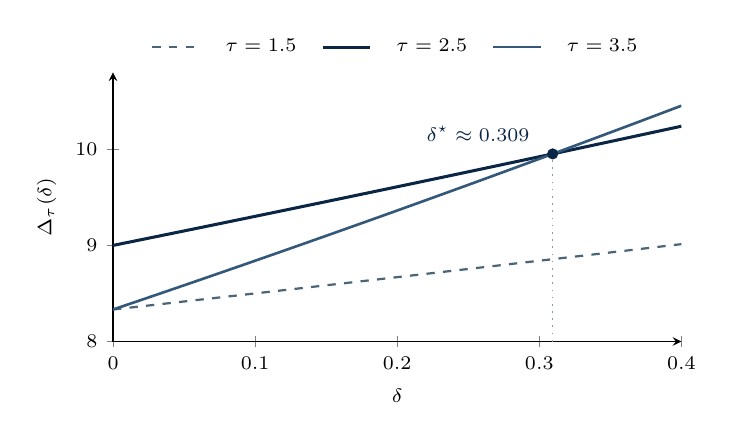
\begin{tikzpicture}
\begin{axis}[
  width=8.8cm,height=5.0cm,
  axis lines=left,
  xlabel={$\delta$},ylabel={$\Delta_\tau(\delta)$},
  xmin=0,xmax=0.4,ymin=8.0,ymax=10.8,
  xtick={0,0.1,0.2,0.3,0.4},
  ytick={8,9,10},
  tick label style={font=\scriptsize},
  label style={font=\scriptsize},
  legend style={draw=none,font=\scriptsize,at={(0.5,1.02)},anchor=south,
    legend columns=3,column sep=0.7em},
]
\addplot[domain=0:0.4,samples=80,draw=steel,line width=0.8pt,dashed]{(10+x)^2/12};
\addlegendentry{$\tau=1.5$}
\addplot[domain=0:0.4,samples=80,draw=navy,line width=1.1pt]{(3+x/2)^2};
\addlegendentry{$\tau=2.5$}
\addplot[domain=0:0.4,samples=80,draw=navy2,line width=0.95pt]{0.75*(10/3+x)^2};
\addlegendentry{$\tau=3.5$}
\draw[dotted,steel!65,line width=0.6pt] (axis cs:0.3094,8.0) -- (axis cs:0.3094,9.952);
\addplot[only marks,mark=*,mark size=1.8pt,draw=navy,fill=navy] coordinates {(0.3094,9.952)};
\node[font=\scriptsize,text=navy,anchor=south east] at (axis cs:0.30,9.98) {$\delta^\star\approx0.309$};
\end{axis}
\end{tikzpicture}
\caption{例 B 的切分翻转。三条线是三个候选阈值的根增益随 $\delta$ 的变化；中间与最右两刀在 $\delta^\star\approx0.309$ 处交叉。左侧 $\tau=2.5$ 最优，右侧 $\tau=3.5$ 最优；$\tau=1.5$ 始终最低。}
\label{fig:flip}
\end{figure}

\paragraph{偏差与方差} 上面的翻转是「同一份数据、换一个响应值」的敏感度。更常见的问法是「换一批样本，预测会变多少」。把这两件事分开，需要偏差—方差分解。

在平方损失下，固定测试输入 $\bx$，令 $f^\star(\bx)=\mathbb E[Y\mid\bx]$，写
\[
  Y=f^\star(\bx)+\epsilon,\qquad \mathbb E[\epsilon\mid\bx]=0,\qquad \Var(\epsilon\mid\bx)=\sigma^2 .
\]
训练数据 $\Dcal$ 独立于测试样本抽取，得到 $\widehat f_\Dcal$。展开平方并利用交叉项期望为零：
\begin{equation}
\begin{aligned}
\mathbb E_{\Dcal,\epsilon}\bigl[(Y-\widehat f_\Dcal(\bx))^2\mid\bx\bigr]
={}&\bigl(\mathbb E_{\Dcal}[\widehat f_\Dcal(\bx)]-f^\star(\bx)\bigr)^2
+\Var_{\Dcal}\bigl(\widehat f_\Dcal(\bx)\bigr)\\
&+\Var(\epsilon\mid\bx).
\end{aligned}
\label{eq:biasvar}
\end{equation}
三项依次是偏差平方、预测方差与噪声。

\begin{prop}[偏差—方差分解]
在 $Y=f^\star(\bx)+\epsilon$、$\mathbb E[\epsilon\mid\bx]=0$、$\Dcal$ 与测试样本独立的条件下，\eqref{eq:biasvar} 成立。三项分别度量系统性偏离、跨数据的波动与不可约噪声。
\end{prop}

\begin{proof}
在括号内加减 $\mathbb E_\Dcal[\widehat f_\Dcal(\bx)]$，展开成三项：偏差平方、$(\widehat f-\mathbb E\widehat f)^2$、以及两倍的交叉项。交叉项含因子 $\mathbb E_\Dcal[\mathbb E_\Dcal\hat f-\hat f]=0$，故为零；$\epsilon$ 与 $\Dcal$ 独立，与 $\hat f$ 的交叉项也为零。
\end{proof}

三项各有各的来源。噪声是数据本身的下界，换什么模型都消不掉；偏差来自模型类装不下真函数，树可以通过加深来降；方差来自训练集的抽样波动，树越深越大。剪枝做的事，就是用一点偏差换掉一大块方差。

§3.2 的贪心次优属于\emph{偏差}：固定一份数据，搜索没找到全局最优，这是系统性的。§5.1 的切分翻转属于\emph{方差}：换一份数据，树的结构变了。两者都表现为「树不稳」，但补救办法不同——前者要靠更好的搜索或剪枝，后者要靠平均（下一讲的 bagging）或约束。

\begin{warn}[一次翻转不等于「树不能用」]
单次扰动导致换刀，说明的是 $\argmax$ 在平局附近不连续，不是说这棵树一定泛化差。要判断稳定性，得看多次重抽样的预测分布（§5.1 的 $\Var_\Dcal$），而不是一次实验。反过来，看到一次翻转就断言「树必然过拟合」，也是过度解读。
\end{warn}

\subsection{外推与斜边界}

叶值是常数，所以沿着停留在同一片叶的方向移动，预测不变。例 B 的两叶树桩在 $\tau=2.5$ 处切：$x^{(1)}=-1$ 与 $x^{(1)}=6$ 都在训练范围之外，但落在不同叶，预测分别为 $1$ 与 $4$。再往外走，预测仍是 $1$ 或 $4$——树没有斜率，只有常数。

这是树最硬的一条边界：\emph{它不会外推}。对时间序列、价格、趋势型响应，训练集之外的预测只能是边界叶的值，通常没有意义。线性模型至少会把斜率延伸出去，树连斜率都没有。

第二条边界是斜的边界。取单位正方形、均匀输入，真实边界为 $x^{(2)}=x^{(1)}$。把横轴等分成 $B$ 段，每段用一个水平台阶近似斜线：第 $r$ 段的高度取中点 $(r+1/2)/B$，$r=0,\dots,B-1$。这个构造的误分类概率等于斜线与阶梯夹出的面积：
\begin{equation}
  \sum_{r=0}^{B-1}
  \int_{r/B}^{(r+1)/B}
  \left|u-\frac{r+1/2}{B}\right|\,\dd u
  =B\cdot\frac{1}{4B^2}
  =\frac1{4B}.
  \label{eq:stair}
\end{equation}
每个条带被台阶分成两片叶，共 $2B$ 片叶。所以要让误差降到 $\epsilon$，需要 $B\sim1/(4\epsilon)$ 个条带、$2B$ 片叶。

\begin{figure}[htbp]
\centering
\begin{tikzpicture}[
  st/.style={draw=navy,line width=0.7pt},
  gd/.style={draw=steel!55,line width=0.5pt},
  ax/.style={->,steel!60,line width=0.6pt},
  lb/.style={font=\scriptsize,text=steel,inner sep=2pt},
]
\draw[gd] (0,0) rectangle (5,5);
\draw[gd,dashed] (0,0) -- (5,5);
\foreach \x in {1,2,3,4}{
  \draw[gd,dotted] (\x,0) -- (\x,5);
}
\draw[st] (0,0.5) -- (1,0.5);
\draw[st] (1,1.5) -- (2,1.5);
\draw[st] (2,2.5) -- (3,2.5);
\draw[st] (3,3.5) -- (4,3.5);
\draw[st] (4,4.5) -- (5,4.5);
\draw[ax] (0,0) -- (5.5,0); \node[lb,anchor=west] at (5.5,0) {$x^{(1)}$};
\draw[ax] (0,0) -- (0,5.5); \node[lb,anchor=south] at (0,5.5) {$x^{(2)}$};
\node[font=\scriptsize,text=navy,anchor=west] at (2.15,3.05) {$x^{(2)}=x^{(1)}$};
\node[font=\scriptsize,text=steel,anchor=north] at (2.5,-0.05) {$B=5$ 个条带};
\end{tikzpicture}
\caption{用 5 级水平阶梯逼近斜边界。每个条带内按台阶高度分成两片叶，共 $2B=10$ 片叶；误差是斜线与阶梯之间的面积，等于 $1/(4B)$。}
\label{fig:stair}
\end{figure}

这个 $1/(4B)$ 只针对该边界、该输入分布与这个特定构造，不能外推成「树对斜边界的误差总是 $1/(4B)$」。但它说明了一个量级：轴平行切分逼近斜边界时，叶数随精度线性增长。到 $D$ 维，同样的构造需要 $\epsilon^{-(D-1)}$ 量级的叶数——这就是树在高维退化、随机森林仍需要大量树的几何原因。

\begin{warn}[外推的边界]
树对训练范围之外的输入只给边界叶的值；如果特征会随时间漂移，或者测试集的取值范围超过训练集，预测可能系统性地错。遇到趋势型数据，先把趋势去掉（差分、去时间），再让树学残差；不要指望树自己外推。
\end{warn}

\subsection{不纯度重要性}

树自带一个特征重要性：把某个特征在所有节点上带来的不纯度下降，按节点样本占比加权求和。设 $\Ucal(T)$ 为内部节点集合，$s_t$ 为节点 $t$ 采用的切分，$j_t$ 为所用特征编号，则
\begin{equation}
  \MDI^{(j)}
  =\sum_{t:\,t\in\Ucal(T),\ j_t=j}\frac{N_t}{N}\,\Delta_Q(t,s_t).
  \label{eq:mdi}
\end{equation}
若总下降量为正，可除以 $\sum_{j'}\MDI^{(j')}$ 得到归一化重要性。$N_t/N$ 这个权重说明：同样的节点内增益，在根处比在深处更重要——根处的切分影响全部样本。

MDI 的偏误也来自这个求和。候选阈值多的特征（连续特征、取值多的离散特征）有更多机会在某个节点上碰巧取得大增益；即使它与 $y$ 无关，$\MDI^{(j)}$ 也不会是零。树越深、候选越密，偏误越大。这不是「重要性算错了」，是「在训练集上取最大值」这件事本身有选择偏误。

留出集上的置换重要性可以避开这一点。令 $I_{\mathrm{val}}$ 为留出集索引，$\sigma$ 为这些索引的一个随机排列。固定已训好的模型，只把第 $j$ 维替换为
\[
  \widetilde x_i^{(j)}=x_{\sigma(i)}^{(j)},
\]
其余维度照旧，然后看损失增加多少：
\begin{equation}
  \PI^{(j)}(\sigma)
  =\frac{1}{\lvert I_{\mathrm{val}}\rvert}
   \sum_{i:\,i\in I_{\mathrm{val}}}
   \bigl[L\bigl(y_i,f_T(\widetilde{\bx}_i)\bigr)-L\bigl(y_i,f_T(\bx_i)\bigr)\bigr].
  \label{eq:pi}
\end{equation}
重复置换若干次取平均，得到该特征的置换重要性。它在留出集上算，模型不变，只破坏第 $j$ 维与响应的对应关系。

两者回答的问题不同。MDI 问「训练时这个特征贡献了多少不纯度下降」，是\emph{样本内}的；PI 问「把这一维打乱，留出损失变多少」，是\emph{样本外}的。相关特征会让两者都失真：MDI 会把同一份证据重复计入两个特征，PI 在打乱一维后另一维还在，损失增加不明显，于是低估。两者都不能当因果效应。

\begin{warn}[不要只用 MDI 做筛选]
MDI 偏向高基数特征，这是选择偏误，不是模型发现了结构。用 MDI 筛特征前，先按特征基数分层看；或者直接用留出集 PI。两者都不同意时，以 PI 为准——它至少是在模型之外测的。
\end{warn}

C2 会做一个对照实验：保留一个有信号的二值特征，加入若干无关的连续特征与无关的二值特征；在训练集上算 MDI，在留出集上做置换，重复若干次记录排名波动。预期是 MDI 把连续特征排得偏高，PI 把无关特征压到接近零。

\begin{keybox}[三条边界，一个来源]
切分不稳定、不能外推、重要性有偏——三件事都来自同一个事实：树只做轴平行切分，叶值是局部常数。知道了来源，就知道哪些补救有效：平均（下一讲的 bagging）降方差，约束（剪枝、$n_{\min}$）降复杂度，换模型（线性、核、神经网络）换掉轴平行这个限制。
\end{keybox}

这一讲停在单棵树上。下一讲从 \eqref{eq:biasvar} 的方差项出发：既然单棵树的方差大，就把许多棵树的预测平均起来。平均为什么有效、需要什么样的树、树之间相关时为什么失效，是 bagging 与随机森林要回答的问题。

% ============================================================
%  习题
% ============================================================

\clearpage
\section*{习题}
\addcontentsline{toc}{section}{习题}
\markboth{习题}{}
\setlength{\parskip}{0.62em}

\subsection*{A 组 · 基础}

\noindent\textbf{A1.} 用例 A 的深度 2 树，走 $x^{(1)}=2$ 与 $x^{(1)}=6$ 两条预测路径，分别报告叶输出与叶内经验概率。再复算根节点的七个候选基尼，以及右支四个候选的加权基尼。

\noindent\textbf{A2.} 列出例 B 的四叶、两叶、单叶三个候选子树的 $R_\lambda$，在 $(0,5)$ 的 $\lambda$ 轴上标出两个交点。解释 $\lambda=13/12$ 为什么没有产生路径跳点。

\noindent\textbf{A3.} 对表 \ref{tab:threemeasures} 的 $(98,2)\to(50,0)\mid(48,2)$，分别用误分类率、基尼、熵算增益。说明三者的差别来自尺子的哪一条性质。

\noindent\textbf{A4.} 写出 \texttt{DecisionTreeClassifier} 的 \texttt{ccp\_alpha} 与本讲 $\lambda$ 的对应关系，并说明分类与回归两种情形下 $R(t)$ 的分母分别是什么。

\subsection*{B 组 · 提高}

\noindent\textbf{B1.} 推导回归切分恒等式
\[
  \Delta_{\SSE}=\frac{N_{t_L}N_{t_R}}{N_t}(\bar y_{t_L}-\bar y_{t_R})^2 .
\]
再用凹性证明：把一块区域加细划分，加权基尼不纯度不会上升。

\noindent\textbf{B2.} 用异或数据检验正增益门槛：写出 $\gamma>0$ 与 $\gamma=0$ 两种设置下的树与训练误差。再对例 B 穷举三个三叶划分，比较贪心与全局最优。说明这两小题分别检验了生长规则的哪一步。

\noindent\textbf{B3.} 构造一个两类、二维的例子，使某次切分的基尼增益为正、熵增益为负。若做不到，说明为什么。

\noindent\textbf{B4.} 证明：在平方损失下，沿同一棵树的生长路径每加一刀，训练 SSE 单调不增。若把叶值固定为切分前的父均值、不重新优化，这个结论还成立吗？

\subsection*{C 组 · 动手}

\noindent\textbf{C1.} 取一份回归数据，固定 $K=5$ 的折分与共同的 $\lambda$ 网格。对每个 $\lambda$ 记录平均验证误差与平均叶数，画两条曲线，标出 $\lambda_{\min}$ 与 $\lambda_{\mathrm{1SE}}$，最后在留出测试集上报告两个 $\lambda$ 的测试误差。

\noindent\textbf{C2.} 生成一份数据：一个与响应有信号的二值特征，加上若干无关的连续特征与无关的二值特征。训练一棵足够深的树，记录训练集 MDI 排名；在留出集上做 20 次置换重要性，记录排名波动。比较两种排名对无关特征的处置。

\subsection*{提示}

\begin{itemize}[itemsep=0.2em]
  \item \textbf{A1}：$x^{(1)}=2$ 落左叶 $(3,0)$，类 0，概率 $1$；$x^{(1)}=6$ 落中间叶 $(1,2)$，类 1，概率 $2/3$，真实标签为 0。根候选为 $3/7,1/3,1/5,3/8,7/15,1/3,3/7$；右支为 $3/10,4/15,4/15,3/10$。
  \item \textbf{A2}：四叶 $0+4\lambda$，两叶 $1+2\lambda$，单叶 $13/4+\lambda$；交点在 $\lambda=1/2$ 与 $9/4$。$\lambda=13/12$ 时两叶为 $19/6\approx3.17$，四叶与单叶都是 $13/3\approx4.33$，两叶已经最优。
  \item \textbf{A3}：误分类率的增益为 $0$，基尼 $0.0008$，熵 $0.0203$ bit。差别来自 $\Err$ 只看多数类，$G$ 与 $H$ 是严格凹的，对「置信度提高」也给正分。
  \item \textbf{A4}：\texttt{ccp\_alpha} 就是 $\lambda$；分类的 $R(t)=(N_t/N)Q(\widehat{\bp}_t)$，回归的 $R(t)=\SSE(t)/N$。两者都除以总样本数 $N$。
  \item \textbf{B1}：对两个孩子各用一次平方和恒等式，再用 $N_t\bar y_t=N_{t_L}\bar y_{t_L}+N_{t_R}\bar y_{t_R}$ 消去 $\bar y_t$。凹性用 Jensen：$\widehat{\bp}_t$ 是子节点频率的凸组合。
  \item \textbf{B2}：异或首切两侧都是 $(1/2,1/2)$，$\Delta_G=\Delta_H=0$；$\gamma>0$ 停在根，误差 $1/2$；$\gamma=0$ 允许首切，两个子节点再切另一维，误差 $0$。例 B 的三个切点对给出 SSE $2,0.5,2$。前者检验停止规则，后者检验搜索步骤。
  \item \textbf{B3}：做不到。熵与基尼都是凹的，且在任何切分上增益非负（§2.4 的 Jensen）；差别只在数值，不在符号。
  \item \textbf{B4}：成立，因为每一刀都可以选择不切（增益 $0$），切了之后叶值只会更优。若固定叶值不重新优化，切分仍可能降低 SSE（把样本分到更合适的固定值），但「不切」仍是合法选项，所以单调性仍成立；只是增益公式要改。
  \item \textbf{C1}：用 \texttt{cost\_complexity\_}\allowbreak\texttt{pruning\_path} 取候选 $\alpha$，对每个 $\alpha$ 在验证折上算误差；共同网格取各折 $\alpha$ 的并集。叶数用 \texttt{get\_n\_leaves()}，1-SE 阈值用折间标准误。
  \item \textbf{C2}：\texttt{feature\_importances\_} 是 MDI；\texttt{permutation\_}\allowbreak\texttt{importance} 在留出集上做，重复 $20$ 次。预期连续噪声特征的 MDI 排名偏高，PI 均值接近 $0$，方差更大。
\end{itemize}

% ============================================================
%  附录
% ============================================================

\clearpage
\appendix
\renewcommand{\thesection}{\Alph{section}}

\section{公式速查}

\subsection*{A.1　叶值与预测}
\begin{align}
  f_T(\bx)&=\sum_{m\in\Lcal(T)}\theta_m\,\Ind(\bx\in\Rcal_m),&
  \widehat\theta_m&=\bar y_m\ \ (\text{平方损失}),\\
  \widehat\theta_m&\in\argmax_c N_{mc}\ \ (\text{0--1 损失}),&
  \widehat{\bp}_m&=\Bigl(\frac{N_{m0}}{N_m},\dots,\frac{N_{m,C-1}}{N_m}\Bigr).
\end{align}

\subsection*{A.2　不纯度与增益}
\begin{align}
  G(\bp)&=1-\sum_c p_c^2,&
  H(\bp)&=-\sum_c p_c\log_2 p_c,\\
  \Err(\bp)&=1-\max_c p_c,&
  \Delta_Q(t,s)&=Q(\widehat{\bp}_t)
    -\frac{N_{t_L}}{N_t}Q(\widehat{\bp}_{t_L})
    -\frac{N_{t_R}}{N_t}Q(\widehat{\bp}_{t_R}),\\
  \Delta_{\SSE}(t,s)&=\frac{N_{t_L}N_{t_R}}{N_t}(\bar y_{t_L}-\bar y_{t_R})^2 .
\end{align}

\subsection*{A.3　快速 SSE 与剪枝}
\begin{align}
  \SSE(t)&=\sum_{i\in I_t}y_i^2-\frac{\bigl(\sum_{i\in I_t}y_i\bigr)^2}{N_t},&
  R(T)&=\sum_{m\in\Lcal(T)}R(m),\\
  R_\lambda(T)&=R(T)+\lambda\lvert T\rvert,&
  \lambda_t&=\frac{R(t)-R(T_t)}{\lvert T_t\rvert-1}.
\end{align}

\subsection*{A.4　交叉验证与 1-SE}
\begin{align}
  \bar E(\lambda)&=\frac1K\sum_{k=1}^K E_k(\lambda),&
  \widehat{\mathrm{SE}}(\lambda)&=\sqrt{\frac{\sum_k[E_k(\lambda)-\bar E(\lambda)]^2}{K(K-1)}},\\
  \lambda_{\min}&=\argmin_{\lambda\in\Lambda}\bar E(\lambda),&
  \lambda_{\mathrm{1SE}}&=\max\{\lambda\in\Lambda:\bar E(\lambda)\le
    \bar E(\lambda_{\min})+\widehat{\mathrm{SE}}(\lambda_{\min})\}.
\end{align}

\subsection*{A.5　除以谁：$N_t$ 还是 $N$}
\begin{center}
\small
\begin{tabular}{@{}lll@{}}
\toprule
\rowcolor{navy!7}
\tabhead 量 & \tabhead 分母 / 尺度 & \tabhead 说明\\
\midrule
$\widehat p_{tc},\ G,\ H,\ \Err$ & $N_t$ & 节点内频率与不纯度\\
$\bar y_t,\ \SSE(t)$ & $N_t$ & 节点内均值与平方和\\
$R(t)$ & $N$ & 该叶对整树风险的贡献\\
$R(T),\ R_\lambda(T)$ & $N$ & 整树风险；$\lambda$ 与它同尺度\\
$\Delta_Q(t,s)$ & 无量纲 & 父与子的加权差\\
$\MDI^{(j)}$ & $N$ & 权重 $N_t/N$，不是 $N_t/N_t$\\
\bottomrule
\end{tabular}
\end{center}

\section{延伸阅读}

\begin{enumerate}[label={[\arabic*]},leftmargin=2.6em,itemsep=0.45em]
  \item L. Breiman, J. Friedman, R. Olshen, C. Stone. \emph{Classification and Regression Trees}. Wadsworth, 1984.\\[1pt]
  {\footnotesize\color{steel}CART 的原始著作。代价复杂度剪枝、最弱环节、下包络的完整推导都在第 3 章与第 10 章；本讲 §4.2 的记号按这本书的写法统一。}

  \item J. R. Quinlan. \emph{C4.5: Programs for Machine Learning}. Morgan Kaufmann, 1993.\\[1pt]
  {\footnotesize\color{steel}信息增益率、连续特征二分、缺失值处理的出处。连续属性的系统讨论另见 \url{https://arxiv.org/abs/cs/9603103}。}

  \item T. Hastie, R. Tibshirani, J. Friedman. \emph{The Elements of Statistical Learning}, 2nd ed., ch.~9. Springer, 2009.\\[1pt]
  {\footnotesize\color{steel}教材处理：树的偏差—方差、剪枝、变量重要性。§9.2 的图与本讲 §4.1 的训练/验证曲线是同一个意思。}

  \item C. Strobl, A.-L. Boulesteix, A. Zeileis, T. Hothorn. Bias in random forest variable importance measures. \emph{BMC Bioinformatics}, 8:25, 2007.\\[1pt]
  {\footnotesize\color{steel}MDI 偏误的系统实验：连续与高基数特征为何占优。§5.3 的结论以此为准。}

  \item W.-Y. Loh. Classification and regression trees. \emph{WIREs Data Mining and Knowledge Discovery}, 1(1):14--23, 2011.\\[1pt]
  {\footnotesize\color{steel}一篇简明的综述，把 ID3、C4.5、CART、CHAID 的差别放在同一张表里。适合与 §3.3 对照。}

  \item \texttt{scikit-learn} 文档：\texttt{tree} 模块。\\[1pt]
  {\footnotesize\color{steel}\texttt{criterion}、\texttt{min\_samples\_leaf}、\texttt{ccp\_alpha} 与 \texttt{cost\_complexity\_}\allowbreak\texttt{pruning\_path} 的确切含义。§4.2 与 C1 的实现以此为准。}
\end{enumerate}

\vspace{1.0em}
\begin{flushright}
{\color{navy!25}\rule{3.2cm}{0.5pt}}\\[5pt]
{\footnotesize\color{steel}第六讲 · 完}
\end{flushright}

\end{document}
